\documentclass[aspectratio=169,xcolor=dvipsnames]{beamer}
\usetheme{SimpleDarkBlue}
\usepackage{textcomp}

\usepackage{hyperref}
\usepackage{subfig}
\usepackage{gensymb}
\usepackage{xcolor}

\usepackage{graphicx} % Allows including images
\usepackage{booktabs} % Allows the use of \toprule, \midrule and \bottomrule in tables
\renewcommand{\indent}{\hspace*{2em}}



\hypersetup{
    colorlinks=true,
    linkcolor=blue,
    urlcolor=blue,
    citecolor=blue
}


%-TITLE-PAGE-------------------------------------------

\title{LoRA}

\author{Yuchen Yan}
\institute{Australian National University}
\date{\today}

%------------------------------------------------------

\begin{document}

\begin{frame}
    \titlepage
\end{frame}

\begin{frame}{Overview}
    \tableofcontents
\end{frame}

%------------------------------------------------
\section{LoRA Problem Statement}
%------------------------------------------------

\begin{frame}{Problem statement - conditional language modeling objective}
    Fine tuning, the model is initialized to pre-trained weights $\Phi{0}$ and updated to $\Phi_{0} + \Delta \Phi$ by repeatedly following the gradient to maximize the conditional language modeling objective:
    \begin{align*}
        \max _{\Phi} \sum_{(x, y) \in \mathcal{Z}} \sum_{t=1}^{|y|} \log \left(P_{\Phi}\left(y_t \mid x, y_{<t}\right)\right)
    \end{align*}

    \begin{itemize}
        \item $\mathcal{Z}$ the training dataset of input-output pairs $(x,y)$
        \item $y_{<t}$ all tokens before timestep $t$
        \item $P_{\Phi}\left(y_t \mid x, y_{<t}\right)$ the model's predicted probability of the token $y_t$, given the input $x$ and previously generated tokens $y_{<t}$
    \end{itemize}
\end{frame}

%------------------------------------------------
\section{Parameter efficient approach}
%------------------------------------------------

\begin{frame}{Parameter efficient approach}
    Adopt a more parameter-efficient approach, where the task-specific parameter increment $\Delta \Phi=\Delta \Phi(\Theta)$ is further encoded by a much smaller-sized set of parameters $\Theta$ with $|\Theta| \ll\left|\Phi_0\right|$. The task of finding $\Delta \Phi$ thus becomes optimizing over $\Theta$ :
    \bigskip
    \begin{align*}
        \max _{\Theta} \sum_{(x, y) \in \mathcal{Z}} \sum_{t=1}^{|y|} \log \left(p_{\Phi_0+\Delta \Phi(\Theta)}\left(y_t \mid x, y_{<t}\right)\right)
    \end{align*}
\end{frame}

%------------------------------------------------
\section{Existing solutions}
%------------------------------------------------

\begin{frame}{Existing solutions-Adapter}
    \begin{columns}
        \begin{column}{0.7\textwidth}
            \begin{figure}
                \centering
                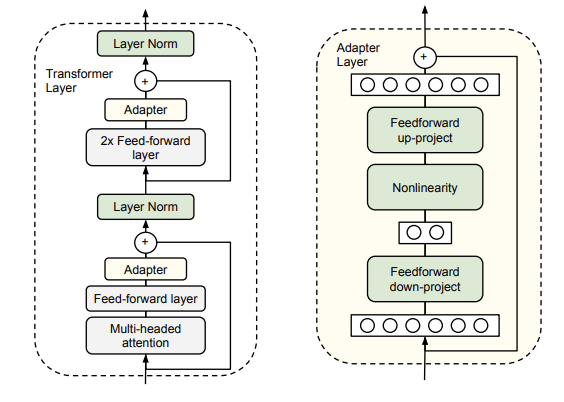
\includegraphics[width=0.9\linewidth]{figures/adapter_architecture.png}
            \end{figure}
        \end{column}
        \begin{column}{0.3\textwidth}
            Two adapter layers per Transformer block with bottleneck architecture to limit the number of parameters
            \begin{align*}
                |\Theta| = 2md + d + m
            \end{align*}
            $md$ for projection, $m$ for up-projection bias and $d$ for down-projection bias
        \end{column}
    \end{columns}
\end{frame}

%------------------------------------------------

\begin{frame}{Existing solutions- Adapter Cont.}
    \begin{columns}
        \begin{column}{0.7\textwidth}
            \begin{figure}
            \centering
            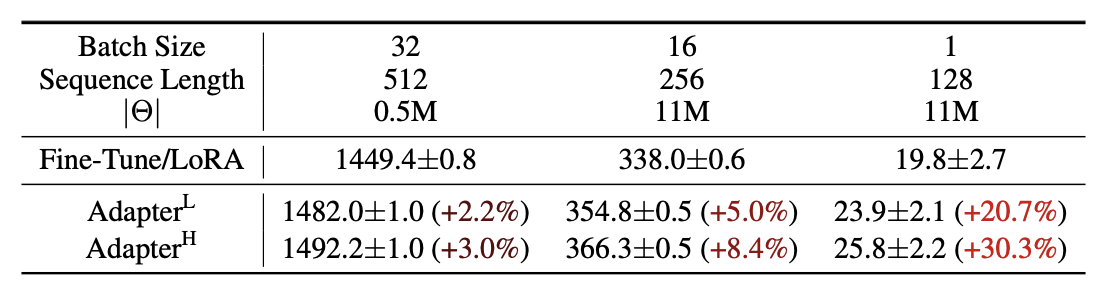
\includegraphics[width=0.8\linewidth]{figures/adapter_latency.png}
            \end{figure}
            \begin{figure}
            \centering
            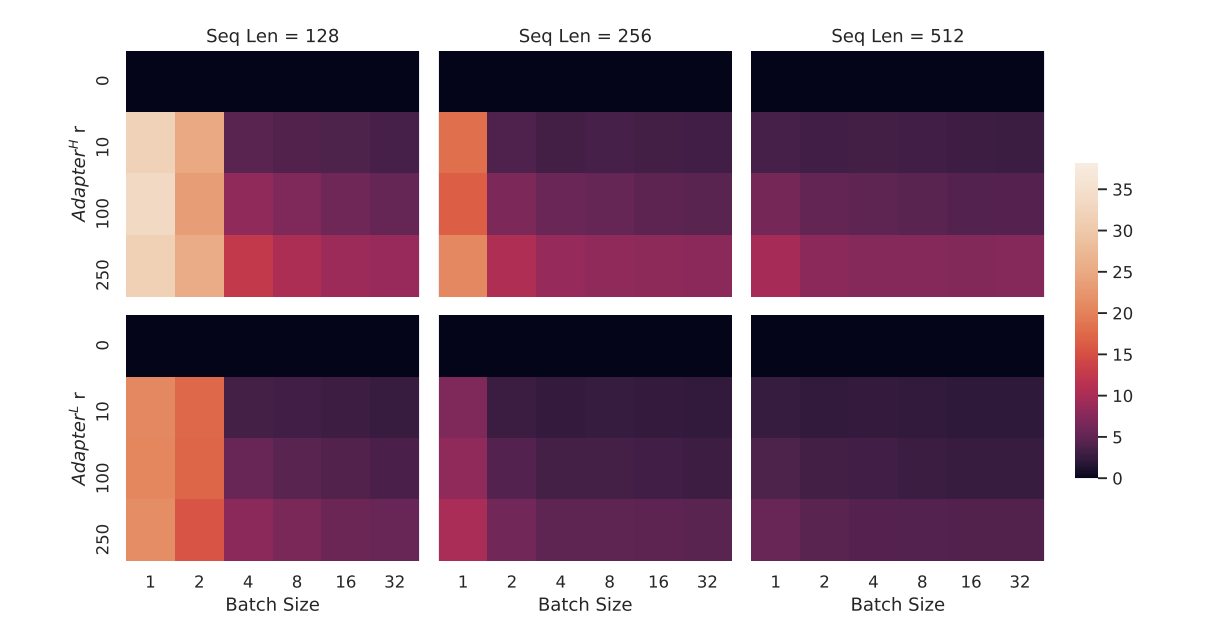
\includegraphics[width=0.9\linewidth]{figures/adapter_parallelsim_latency.png}
            \end{figure}
        \end{column}
        \begin{column}{0.3\textwidth}
            Adapters are added sequentially, without hardware parallelism (online inference scenario), a significant increase in latency 
        \end{column}
    \end{columns}
\end{frame}

%------------------------------------------------

\begin{frame}{Existing solutions-Prefix tuning \& Limitation}
    \begin{columns}
        \begin{column}{0.7\textwidth}
            \begin{figure}
                \centering
                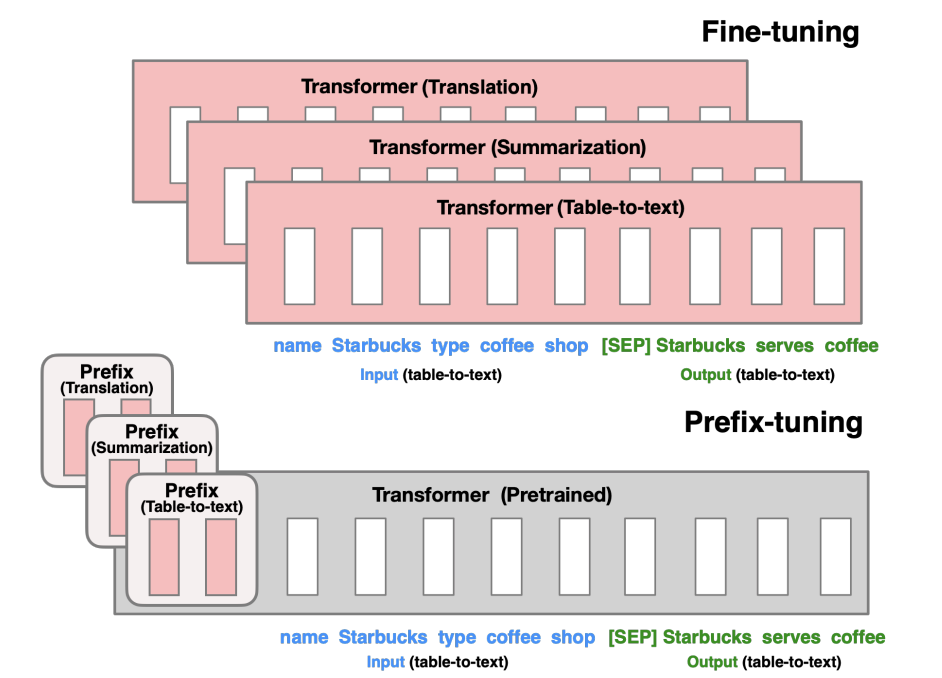
\includegraphics[width=0.9\linewidth]{figures/prefix_tuning_architecture.png}
            \end{figure}
        \end{column}
        \begin{column}{0.3\textwidth}
           Prepends a sequence of \textit{continuous task-specific} vectors to the input, only prefix is optimized. \\
           \bigskip
           \textbf{Limitation} difficult to optimize and adapted reduced sequence length for application
        \end{column}
    \end{columns}
\end{frame}




%------------------------------------------------
\section{Low-rank Adaptation}
%------------------------------------------------

\begin{frame}{Low-rank-parametrized Update Matrices}
    \begin{columns}
        \begin{column}{0.3\textwidth}
            \begin{figure}
                \centering
                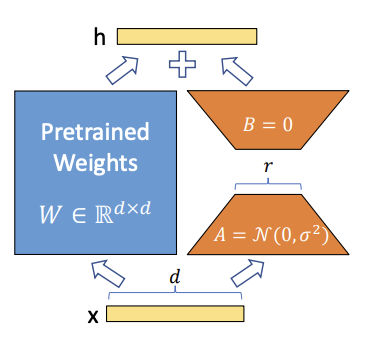
\includegraphics[width=1\linewidth]{figures/LoRA_reparametrization.png}
            \end{figure}
        \end{column}
        \begin{column}{0.7\textwidth}
            \textbf{Inspiration} Aghajanyan et al. (2020) shows that the pre-trained language models have a low "instrisic dimension" and can still learn efficiently despite a random projection to a smaller subspace
        \end{column}
    \end{columns}
\end{frame}

%------------------------------------------------


\begin{frame}{Low-rank-parametrized Update Matrices}
    \textbf{Define}
    For a pre-trained weight matrix         
        \begin{align*}
            W_0 \in \mathbb{R}^{d \times k}
        \end{align*}
        constrains its update by representing the latter with a low-rank decomposition
        \begin{align*}                
            W_0+\Delta W=W_0+B A, 
        \end{align*}
        where $B \in \mathbb{R}^{d \times r}, A \in \mathbb{R}^{r \times k}$ and rank $r \ll \min(d,k)$. \\
        \bigskip
        \textbf{Training}
        $W_0$ is frozen and does not receive gradient updates, while $A$ and $B$ contain trainable parameters. For $h=W_{0} x$, modified forward pass yields:
        \begin{align*}
            h=W_{0} x+\Delta W x=W_{0} x+B A x
        \end{align*}
        \textbf{Initialization} Gaussian for $A$ \& zero for $B$. Scale $\Delta Wx$ by $\alpha/r$ where $\alpha$ is a constant in $r$.  
\end{frame}
%------------------------------------------------


\begin{frame}{Low-rank-parametrized Update Matrices}
    \begin{columns}
        \begin{column}{0.3\textwidth}
            \begin{figure}
                \centering
                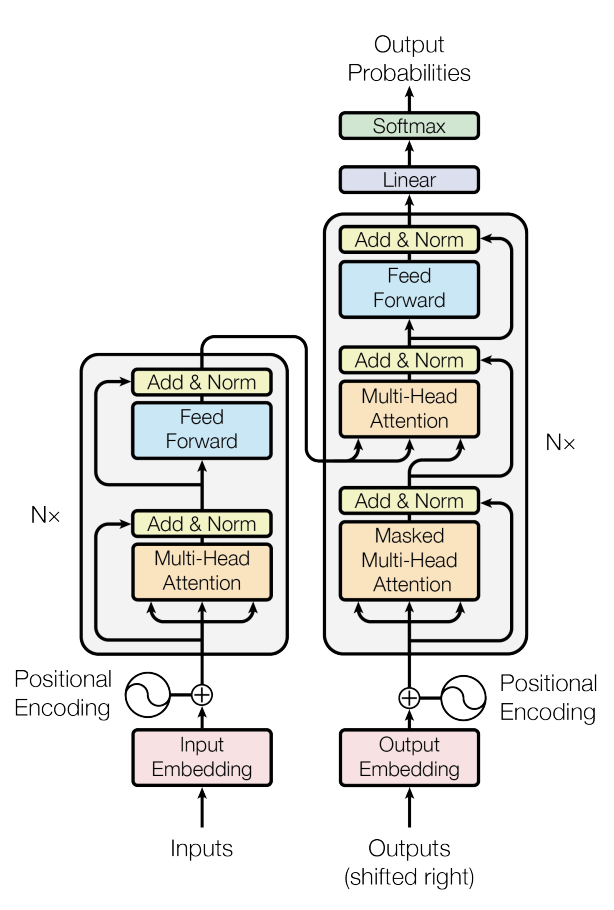
\includegraphics[width=1\linewidth]{figures/transformer_architecture.png}
            \end{figure}
        \end{column}
        \begin{column}{0.7\textwidth}
            \textbf{Application} \\
             LoRA is applicapable to any subset of weight matrices.\\
             \bigskip
            
             \textbf{Transformer} \\
            four weight matrices in the self-attention module ( $W_{q}, W_{k}, W_{v}, W_{o}$ ) and two in the MLP module. \\
            \bigskip
            
            \textbf{Benefits}\\
            \begin{itemize}
                \item reduction in memory and storage usage
                \item switch between tasks at a much lower cost by only swapping the LoRA weights
            \end{itemize}
            \bigskip    
            
            \textbf{Limitation}\\
            Not straightforward to batch inputs to different tasks
        \end{column}
    \end{columns}
\end{frame}



%------------------------------------------------
\subsection{Experiments}
%------------------------------------------------

\begin{frame}{General Language Understanding Evaluation (GLUE)}
    GLUE is a multitask benchmark and analysis platform for natural language understanding.
    \bigskip
    \begin{figure}
        \centering
        \label{GLUE}
        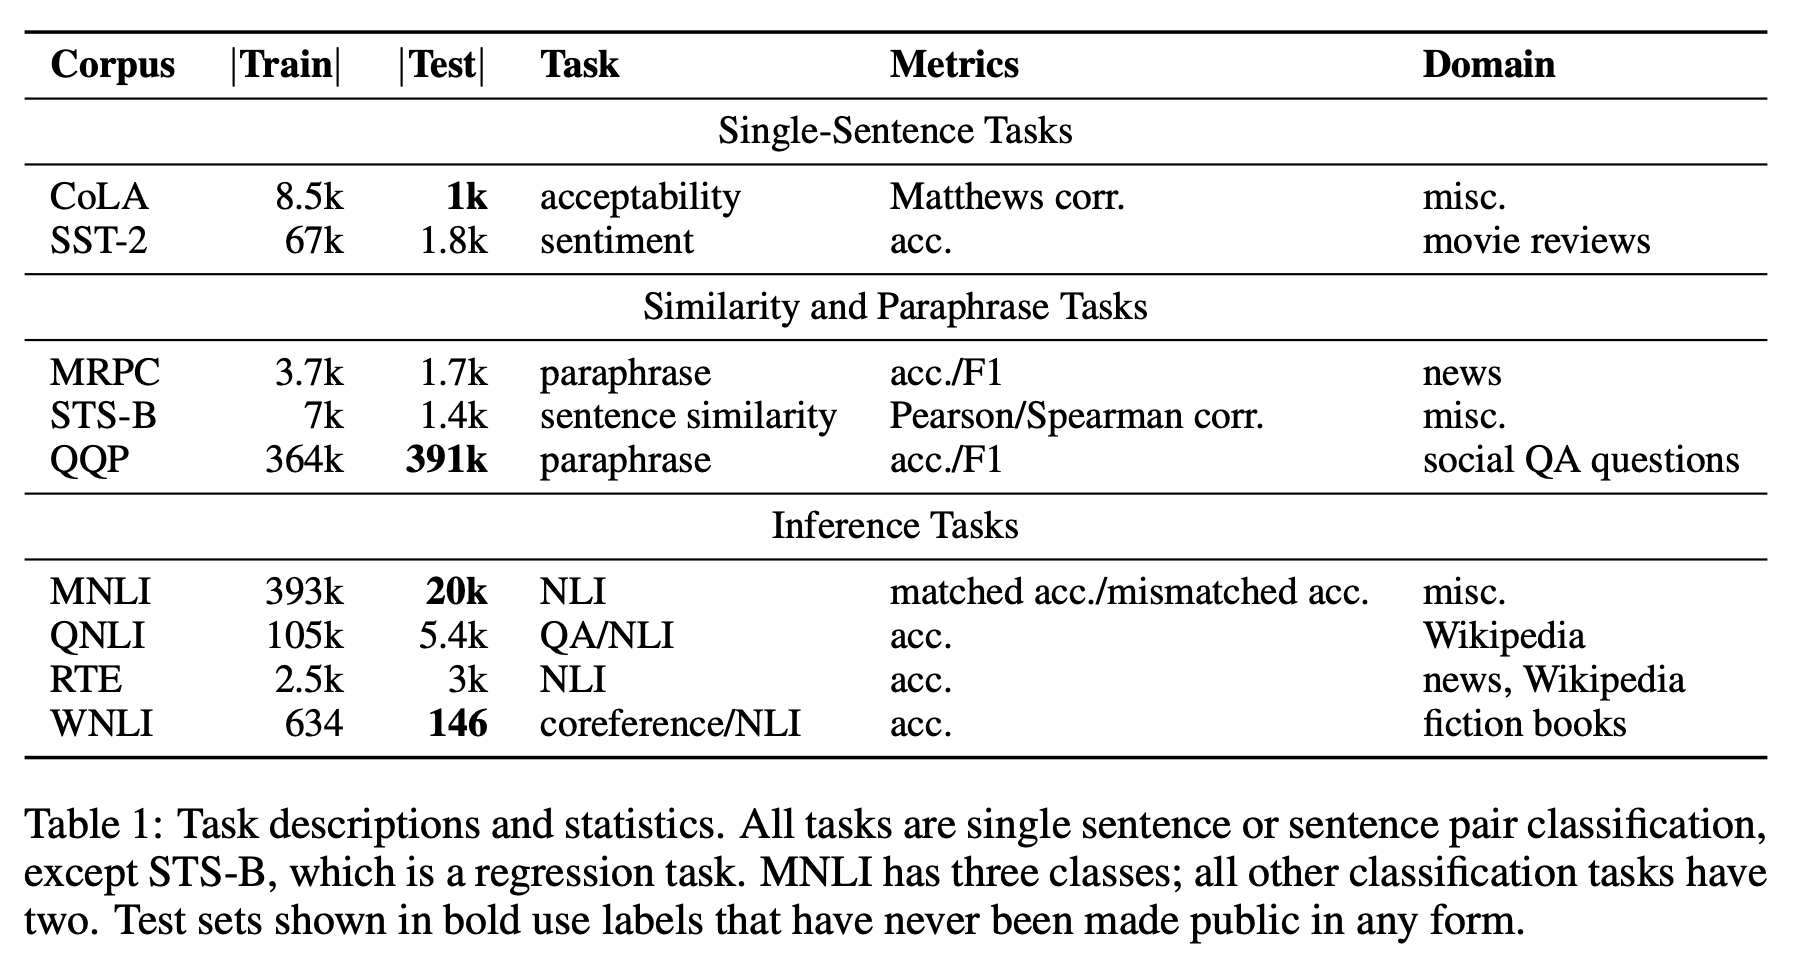
\includegraphics[width=0.8 \linewidth]{figures/GLUE.png}
    \end{figure} 
\end{frame}

%------------------------------------------------

\begin{frame}{Evaluation metrics --- Matthews corr. (CoLA)}
    Matthews correlation coefficient (MCC) as a classification metric
    \bigskip
    \begin{align*}
        \mathrm{MCC}=\frac{(\mathrm{TP} \cdot \mathrm{TN})-(\mathrm{FP} \cdot \mathrm{FN})}{\sqrt{(\mathrm{TP}+\mathrm{FP})(\mathrm{TP}+\mathrm{FN})(\mathrm{TN}+\mathrm{FP})(\mathrm{TN}+\mathrm{FN})}}
    \end{align*}
    $\text{MCC} \in [-1, 1]$\\
    \medskip
    1 $\rightarrow$ perfect prediction\\
    \medskip
    -1 $\rightarrow$ complete disagreement\\
    \medskip
    MCC value is symmetric, the order of the positive and negative classes doesn't matter. \\
    \medskip
    The denominator computes the maximum possible value of the numerator.
\end{frame}

%------------------------------------------------

\begin{frame}{Evaluation metrics ---  Pearson coefficient parameter (STS-B)}
    Pearson coefficient parameter as a metric for linear regression
    \begin{align*}
        r_{x y}=\frac{\sum_{i=1}^n\left(x_i-\bar{x}\right)\left(y_i-\bar{y}\right)}{\sqrt{\sum_{i=1}^n\left(x_i-\bar{x}\right)^2} \sqrt{\sum_{i=1}^n\left(y_i-\bar{y}\right)^2}}
    \end{align*}
        where \\
        - $n$ is sample size \\
        - $x_i, y_i$ are the individual sample points indexed with $i$ \\
        - $\bar{x}=\frac{1}{n} \sum_{i=1}^n x_i$ (the sample mean); and analogously for $\bar{y}$.
\end{frame}

%------------------------------------------------

\begin{frame}[c]{LoRA --- Baselines} 
    \textbf{Fine-Tuning (FT)} the model is initialized to the pre-trained weights and biases, all model parameters undergo gradient updates. One \href{https://arxiv.org/pdf/2101.00190}{baseline} on GPT-2 adapts only last two layers. \\
    \medskip
    \textbf{Bias-only or} \href{https://arxiv.org/abs/2106.10199}{\textbf{BitFit}} only trains the bias vector. \\
    \medskip
    \textbf{Prefix-embedding tuning (\href{https://arxiv.org/abs/2101.00190}{\textbf{PreEmbed}})} inserts special tokens among the input tokens. Use $l_{p}$ (resp. $l_{i}$ ) denote the number of prefix (resp. infix) tokens. $|\Theta|=d_{\text {model }} \times\left(l_{p}+l_{i}\right)$.\\
    \medskip
    \textbf{Prefix-layer tuning (PreLayer)} extension to prefix-embedding tuning. Learns the activations after every Transformer layer. $|\Theta|=L \times d_{\text {model }} \times\left(l_{p}+l_{i}\right)$, where $L$ is the number of Transformer layers.\\
\end{frame}

%------------------------------------------------

\begin{frame}{Evaluation metrics --- Baselines cont.}
    \textbf{Adapter tuning} 
    \begin{itemize}
        \item Adapter${ }^{H}$ Two fully connected layers with biases with a nonlinearity in between.
        \item Adapter${ }^{L}$ Adapter layer applied only after the MLP module and after a LayerNorm.
        \item Adapter${ }^{P}$ similar to $\text{adapter}^L$
        \item Adapter${ }^{D}$ drops some adapter layers for greater efficiency
    \end{itemize}
    \medskip
    In all cases, 
    \begin{align*}
        |\Theta|=\hat{L}_{\text {Adpt }} \times\left(2 \times d_{\text {model }} \times r+r+d_{\text {model }}\right)+2 \times \hat{L}_{L N} \times d_{\text {model }}
    \end{align*}
    where \\
    \begin{itemize}
        \item $\hat{L}_{\text {Adpt }}$ is the number of adapter layers,
        \item $\hat{L}_{L N}$ the number of trainable LayerNorms (e.g., in Adapter ${ }^{\mathrm{L}}$).
    \end{itemize}

    
\end{frame}

%------------------------------------------------
\begin{frame}{LoRA --- Models}
    \begin{itemize}
        \item Natural Language Understanding (NLU)
        \begin{itemize}
            \item RoBERTa, optimised BERT
            \begin{itemize}
                \item pre-trained 125M base
                \item 225M large from HuggingFace Transformers library
            \end{itemize} 
            \item DeBERTa XXL, variant of BERT, 1.5B
        \end{itemize}
        \bigskip
        \item Natural Language Generation (NLG)
        \begin{itemize}
            \item GPT-2 Medium/Large 
            \item GPT-2 175B
        \end{itemize}
    \end{itemize}

\end{frame}

%------------------------------------------------

\begin{frame}{LoRA --- Baselines}
    \begin{figure}
        \centering
        \label{LoRA_baselines}
        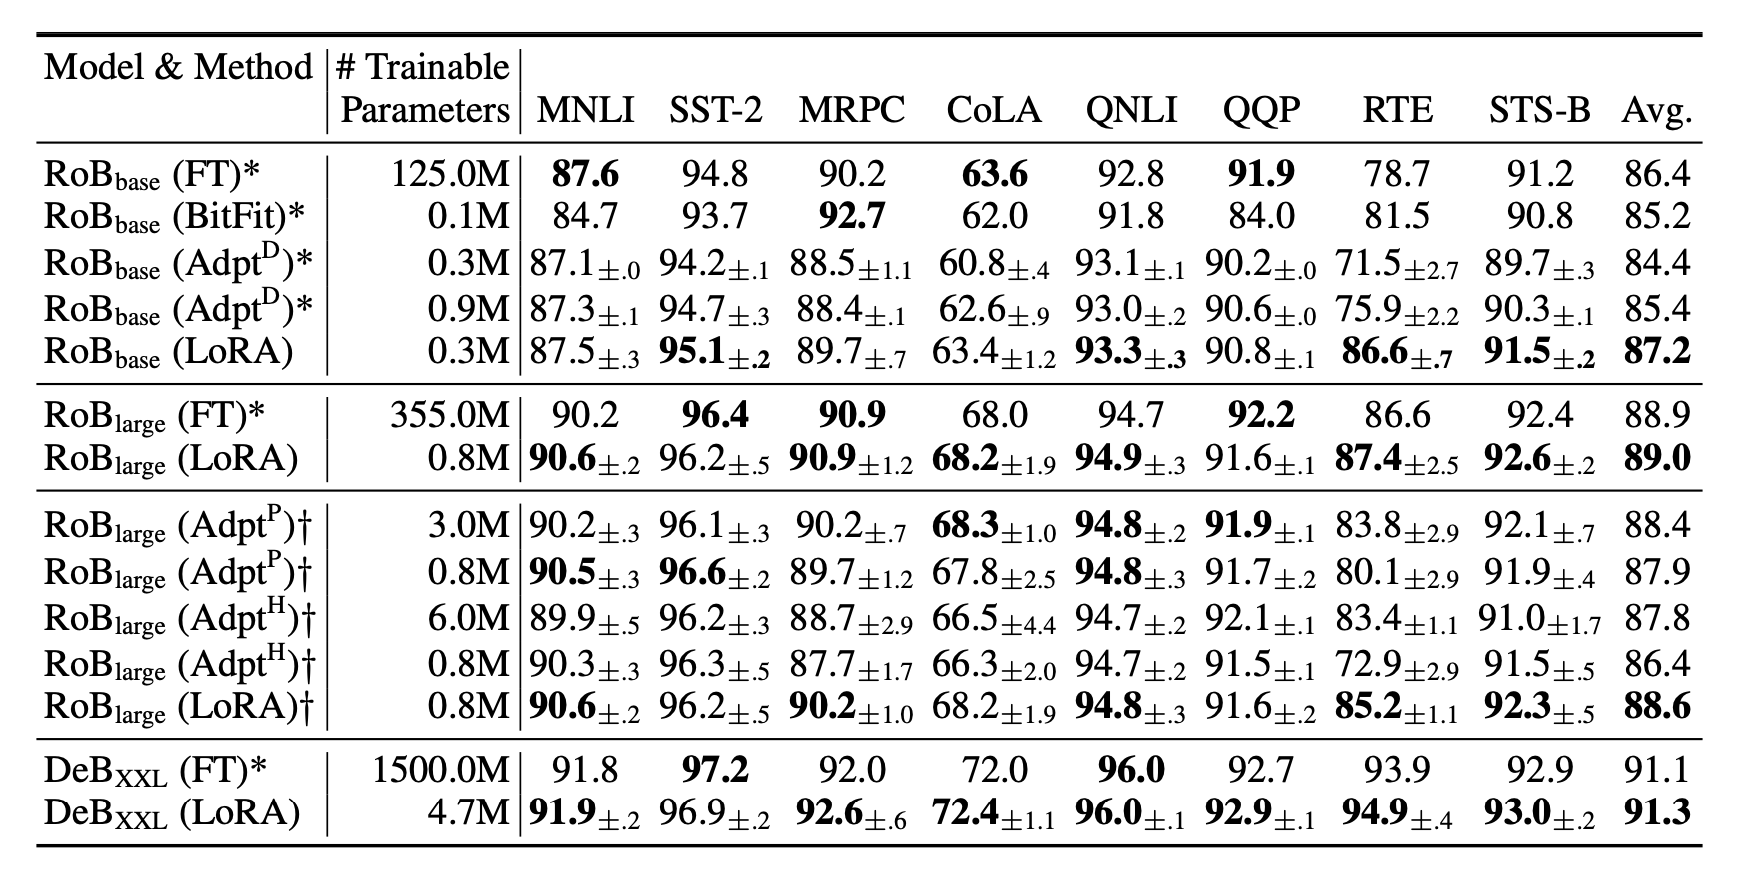
\includegraphics[width=0.8 \linewidth]{figures/baselines.png}
    \end{figure}  
\end{frame}

%------------------------------------------------

\begin{frame}{LoRA --- Baselines}
    \begin{figure}
        \centering
        \label{gpt2_fintune}
        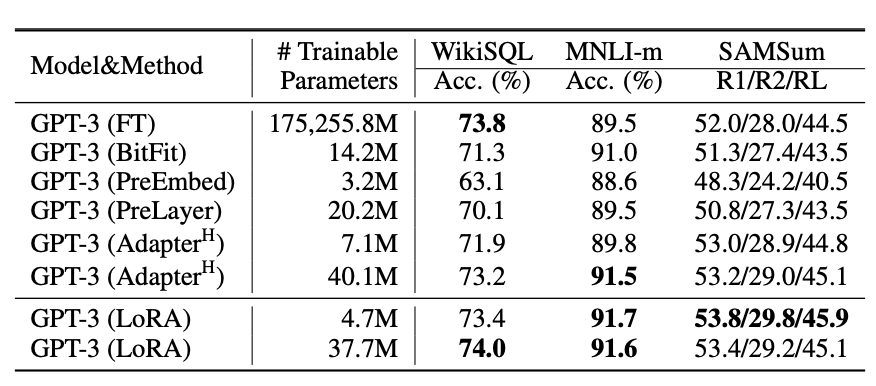
\includegraphics[width=0.8 \linewidth]{figures/gpt2_fintune.png}
    \end{figure}  
\end{frame}

%------------------------------------------------

\begin{frame}{LoRA --- Baselines}
    \begin{figure}
        \centering
        \label{gpt3_finetune}
        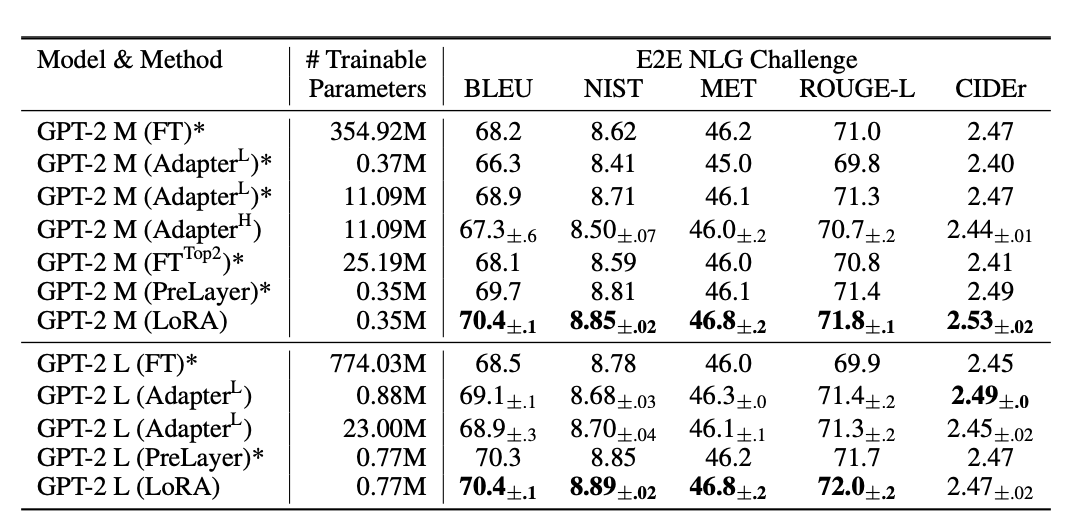
\includegraphics[width=0.8 \linewidth]{figures/gpt3_finetune.png}
    \end{figure}  
\end{frame}

%------------------------------------------------

\begin{frame}{LoRA --- Baselines}
    \begin{figure}
        \centering
        \label{gpt3_performance_parameters}
        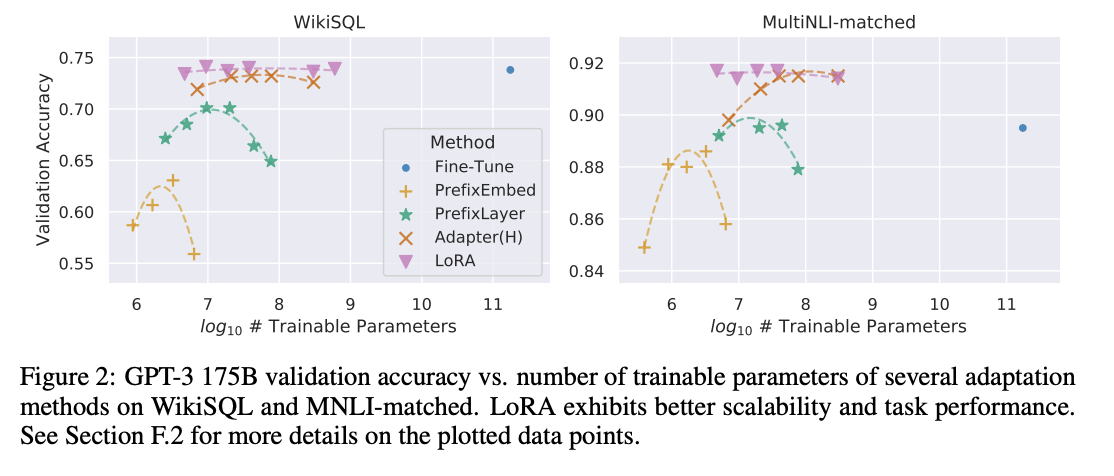
\includegraphics[width=0.8 \linewidth]{figures/gpt3_performance_parameters.png}
    \end{figure}  
\end{frame}

%------------------------------------------------

\begin{frame}{LoRA --- LoRA Advantages}
    \begin{itemize}
        \item lowers the hardware barrier
        \item Better interpretability of correlation between update weights and the pre-trained weights
        \begin{itemize}
            \item GPT-3 175B, the largest reduction of trainable parameters without adversely affecting the task performances
        \end{itemize}
    \end{itemize}
\end{frame}

%------------------------------------------------

\begin{frame}{LoRA --- Understand LoRA updates}
    

    \textbf{Condition}
    \begin{itemize}
        \item Parameter budget constraint 18M
        \item Limited to self -attention module
    \end{itemize}
    \textbf{Eval} The best downstream task performance

    \textbf{Goal} Subsets of weights matrices
\end{frame}

%------------------------------------------------

\begin{frame}{LoRA --- Weight Matrices Selection in Transformer}
    \begin{figure}
        \centering
        \label{budget_parameter}
        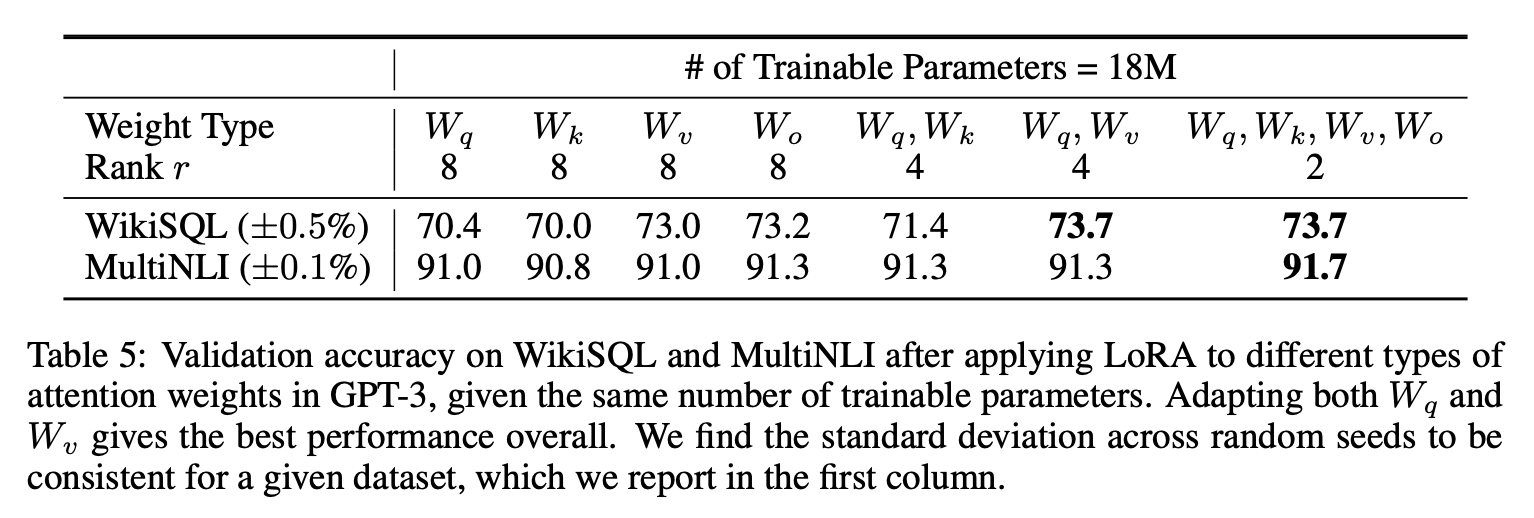
\includegraphics[width=0.8 \linewidth]{figures/budget_parameter.png}
    \end{figure} 
    \textbf{Observations}
    \begin{itemize}
        \item 
    \end{itemize} 
\end{frame}

%------------------------------------------------




\begin{frame}{Image Encoder-Constructing Image Patches}

\begin{columns}
    \begin{column}{0.5\textwidth}
    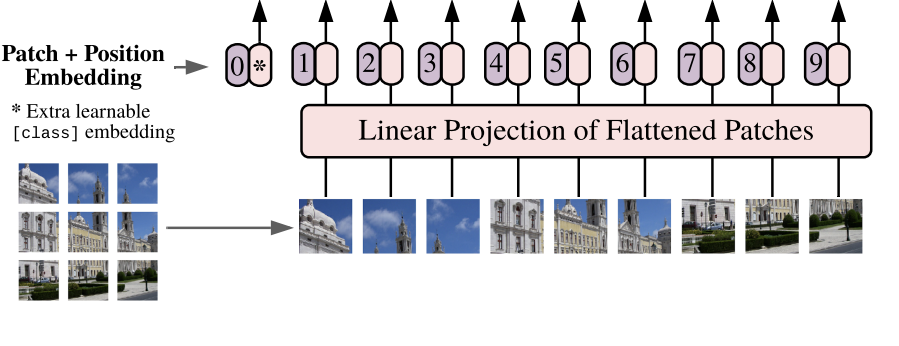
\includegraphics[width=\textwidth]{figures/patches_vision_transformer.png}
    \end{column}

    \begin{column}{0.5\textwidth}
    Reshape the image $x \in \mathbb{R}^{H\times W \times C}$ into a sequence of flattened 2D patches $x_p \in \mathbb{R}^{N\times (P^2\cdot C)}$\\
    \smallskip
    $(H,W) : $ resolution of original image\\
    $C : $ number of channels\\
    $(P,P) : $ resolution of image patch\\
    $N=HW/P^2 : $ number of patches \\
    \bigskip
    Example\\
    $224\times 224$ image with $3$ channels and $16\times 16$ patches,$N=196$
\end{column}
\end{columns}

\end{frame}


%------------------------------------------------

\begin{frame}{Image Encoder --- Linear Projection}

    \begin{columns}
        \begin{column}{0.5\textwidth}
        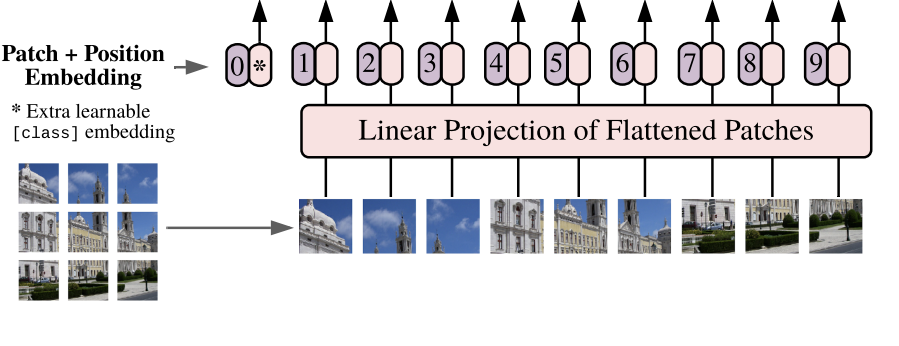
\includegraphics[width=\textwidth]{figures/patches_vision_transformer.png}
        \end{column}
    
        \begin{column}{0.5\textwidth}
        Flatten the patches and map to $D$ dimensions using a trainable linear projection\\
        \begin{align*}
            \mathbf{z}_0
            &=\left[\mathbf{x}_{\text {class }} ; \mathbf{x}_p^1 \mathbf{E} ; \mathbf{x}_p^2 \mathbf{E} ; \cdots ; \mathbf{x}_p^N \mathbf{E}\right]+\mathbf{E}_{p o s}, \\ 
            \bigskip
            &\mathbf{E} \in \mathbb{R}^{\left(P^2 \cdot C\right) \times D}, \\
            &\mathbf{E}_{p o s} \in \mathbb{R}^{(N+1) \times D}
            \end{align*}
        Example\\
        A $16\times 16$ patch with $3$ channels projected to $768$ dimensions, $D=768$
    \end{column}
    \end{columns}
    
    \end{frame}

    
%------------------------------------------------

\begin{frame}{Image Encoder- \texttt{[class]} Token and Position Embeddings}

    \begin{columns}
        \begin{column}{0.5\textwidth}
        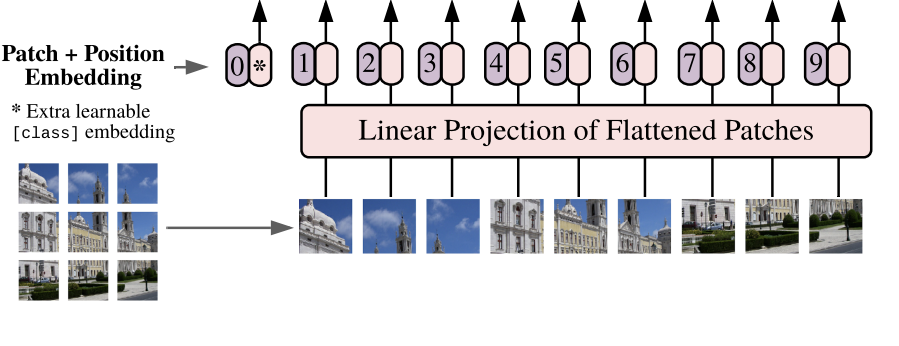
\includegraphics[width=\textwidth]{figures/patches_vision_transformer.png}
        \end{column}
        
        \begin{column}{0.5\textwidth}
        \begin{itemize}
            \item \texttt{[class]} token prepended to the sequence of embedded patches
            \begin{itemize}
                \item interacts with all patches through self-attention, capturing a global summary of the image
                \item acts as the final representation for classification
            \end{itemize}
            \medskip
            \item Position embeddings $\mathbf{E}_{p o s} \in \mathbb{R}^{(N+1) \times D}$
            \begin{itemize}
                \item added to the patch embedding to retain positional information
                \item provide positional information
            \end{itemize}
        \end{itemize}
    \end{column}
    \end{columns}
    \end{frame}
    
    
%------------------------------------------------


\begin{frame}{Self Attention - Layer Normalization}
    \begin{columns}
        \begin{column}{0.25\textwidth}
        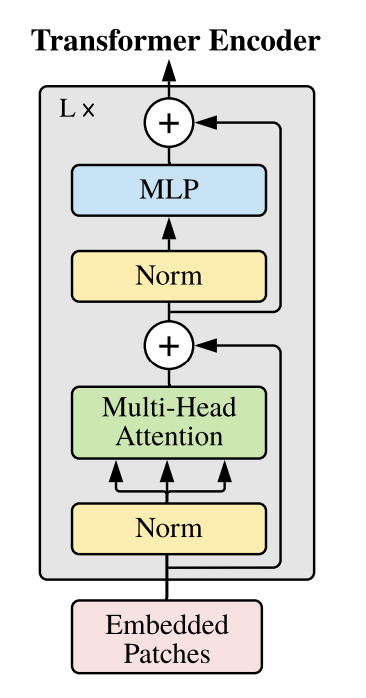
\includegraphics[width=\textwidth]{figures/transformer_encoder.png}
        \end{column}
        \begin{column}{0.6\textwidth}
        Normalize each embedding vector across the channel dimension
        \begin{align*}
            \begin{aligned}
            & \mathrm{LN}(\mathbf{x})=\boldsymbol{\gamma} \odot \frac{\mathbf{x}-\hat{\boldsymbol{\mu}}}{\hat{\boldsymbol{\sigma}}}+\boldsymbol{\beta} . \\
            & \hat{\boldsymbol{\mu}}=\frac{1}{d} \sum_{x^i \in \mathbf{x}} x^i \\
            & \hat{\boldsymbol{\sigma}}^2=\frac{1}{d} \sum_{x^i \in \mathbf{x}}\left(x^i-\hat{\boldsymbol{\mu}}\right)^2+\epsilon \\
            \end{aligned}
            \end{align*}
            $\gamma, \beta \in \mathbb{R}^D$ learnable scale and shift parameters \\
            $\epsilon$ small constant to avoid division by zero \\
        \end{column}
    \end{columns}
\end{frame}

%------------------------------------------------

\begin{frame}{Layer Normalization - Explanation}
    \begin{figure}
        \centering
        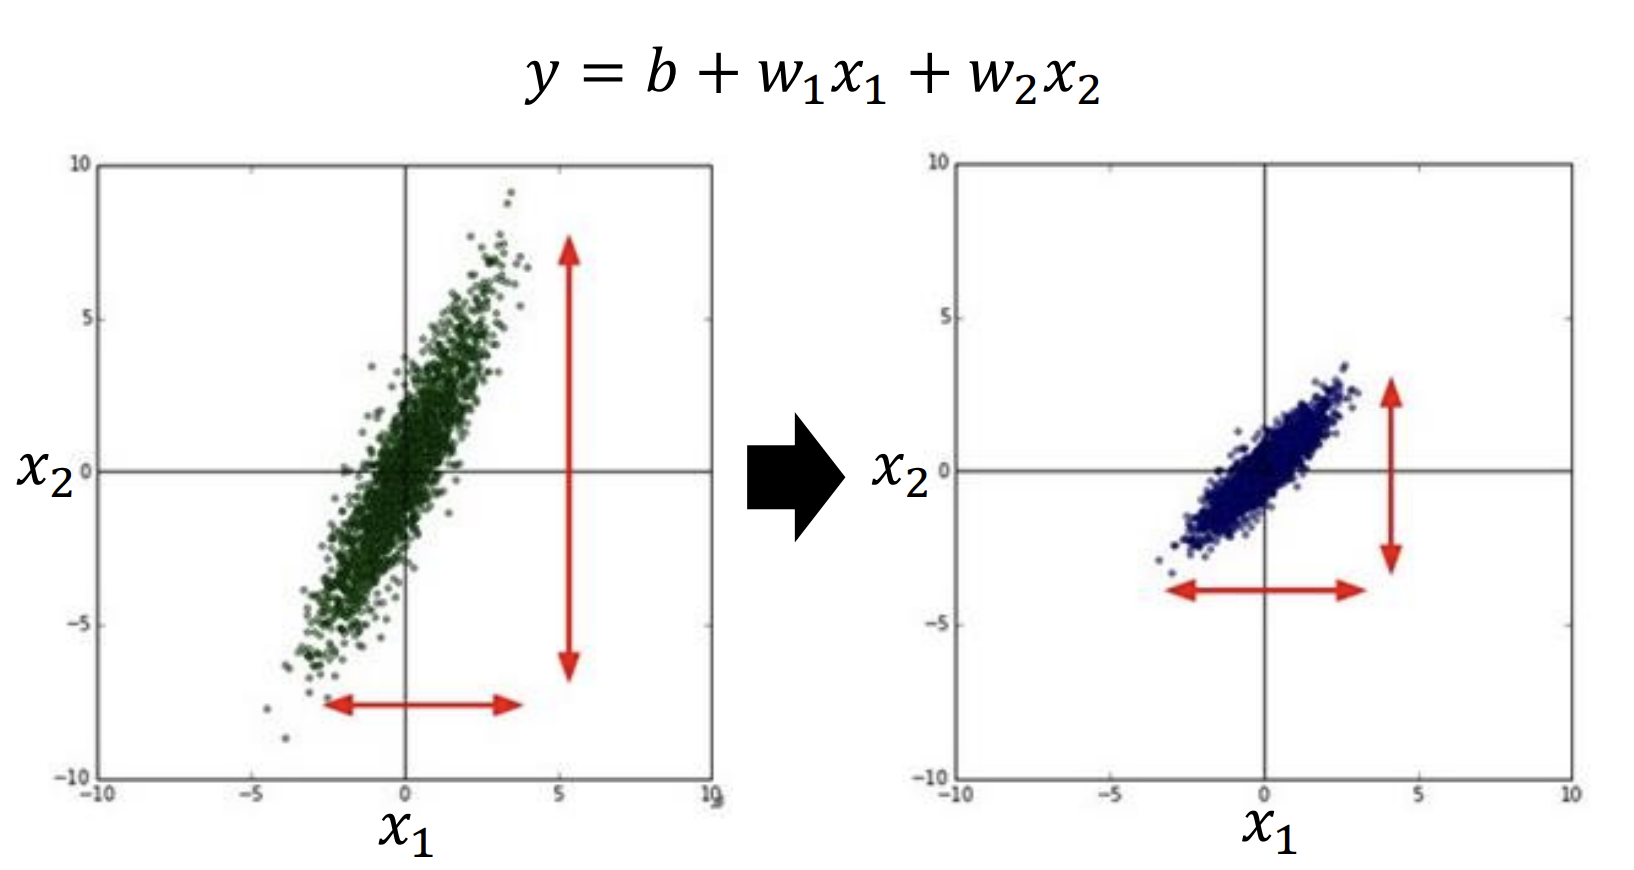
\includegraphics[width=0.8\linewidth]{figures/normalisation.png}
        \label{normalisation}
    \end{figure}
\end{frame}

%------------------------------------------------

\begin{frame}{Layer Normalization - Explanation cont.} 
    \begin{columns}
        \begin{column}{0.65\textwidth}
            \begin{figure}
                \centering
                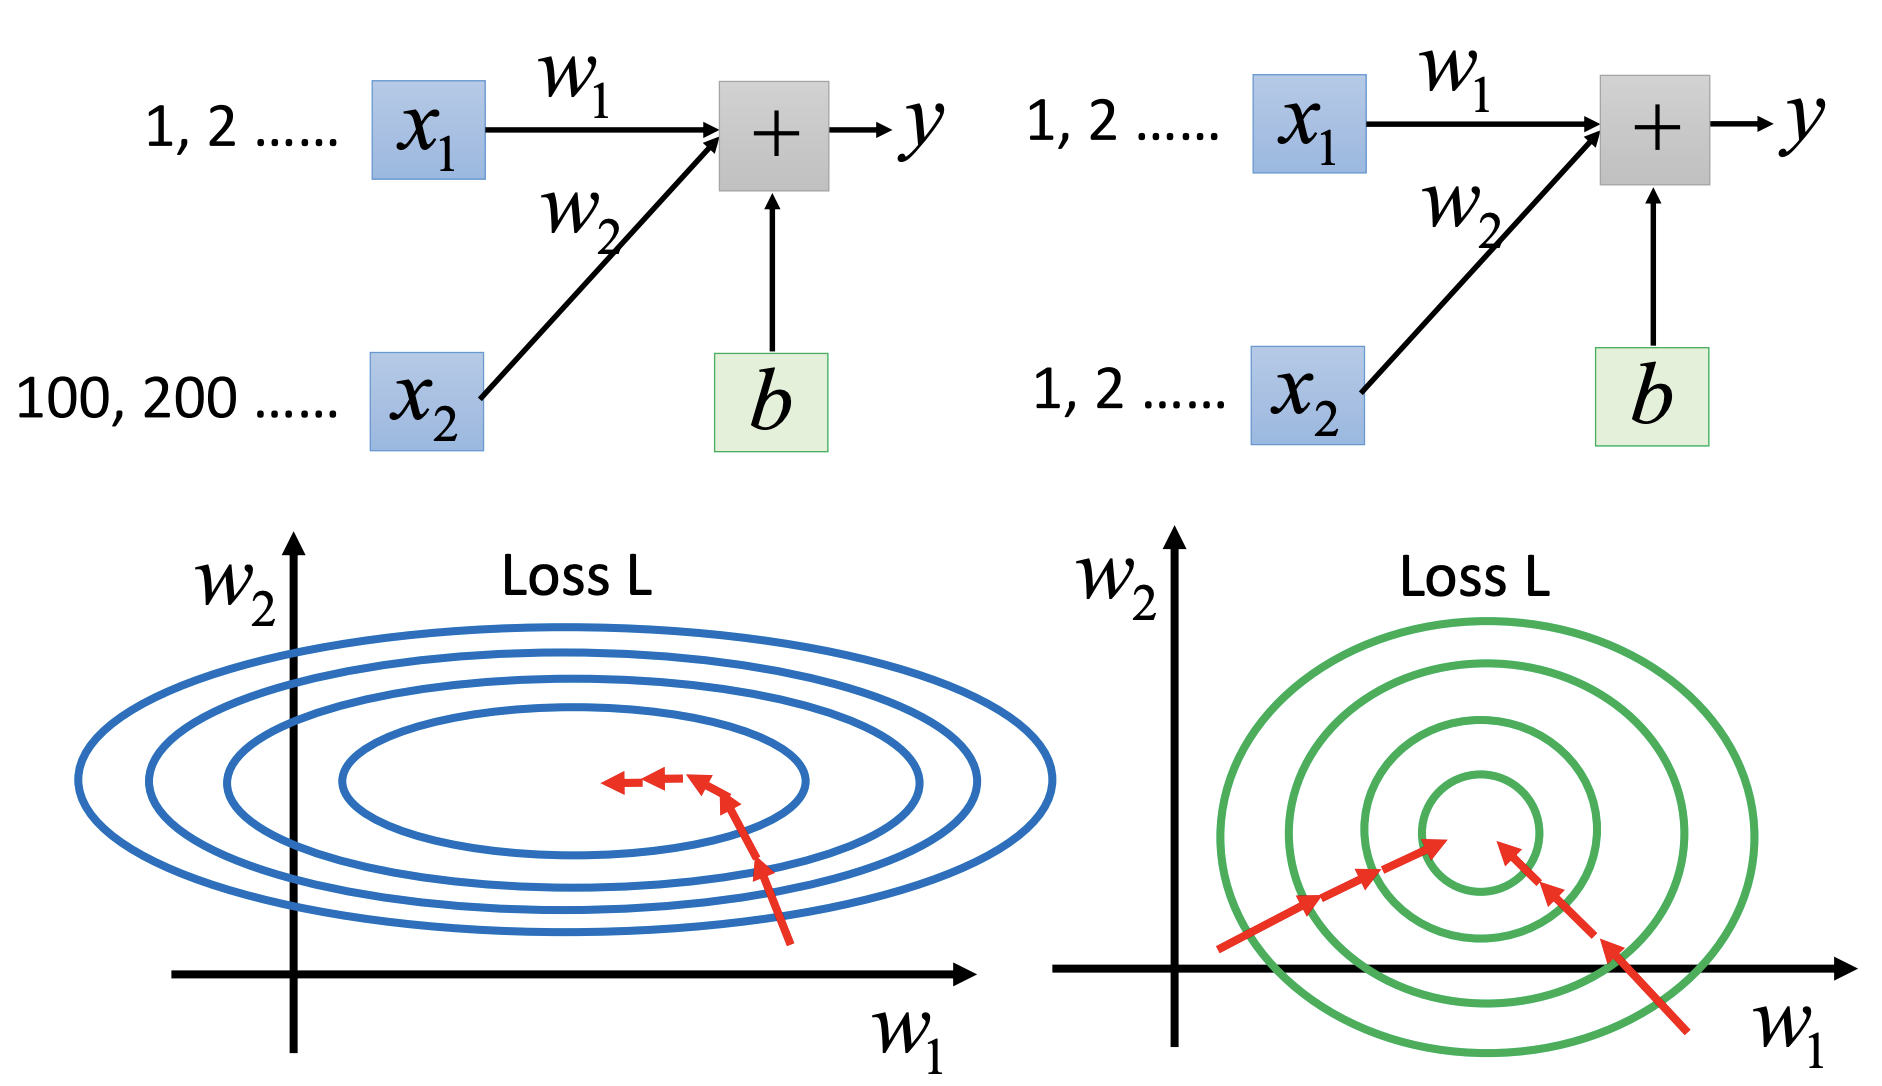
\includegraphics[width=\textwidth]{figures/normalized_gradient_descent.png}
                \label{normalized_gradient_descent}
            \end{figure}
        \end{column}
        \begin{column}{0.35\textwidth}
            \begin{itemize}
                \item Faster convergence
                \item Mitigating interval covariate shift
                \item Reducing the chance of exploding or vanishing gradients
            \end{itemize}
        \end{column}
    \end{columns}
\end{frame}

%------------------------------------------------


\begin{frame}{Image Encoder - Self Attention}
    \begin{columns}
        \begin{column}{0.4\textwidth}
        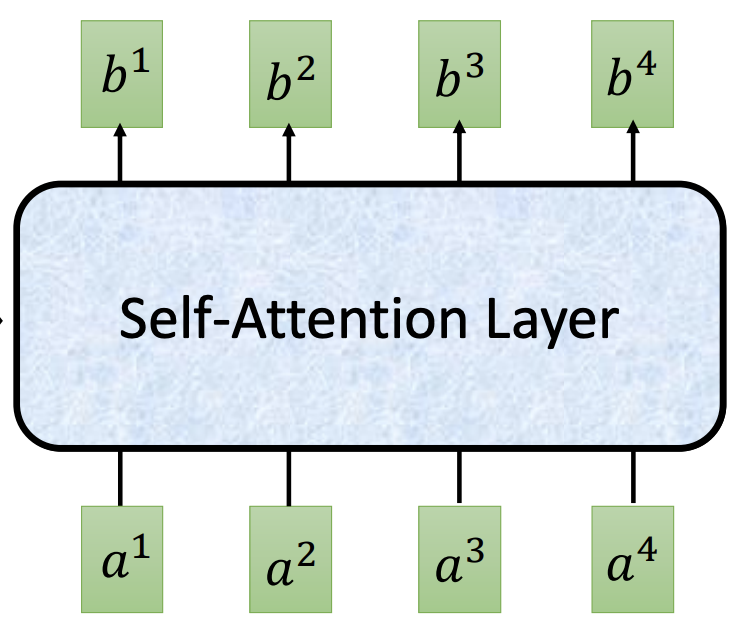
\includegraphics[width=\textwidth]{figures/self_attention.png}
        \end{column}
        \begin{column}{0.6\textwidth}
            \begin{itemize}
                \item $b^i$ is obtained based on the whole input sequence
                \item $b^1,b^2,b^3,b^4$ can be parallelly computed
             \end{itemize}
        \end{column}
    \end{columns}
\end{frame}

%------------------------------------------------

\begin{frame}{Image Encoder - Self Attention}
    \begin{columns}
        \begin{column}{0.6\textwidth}
        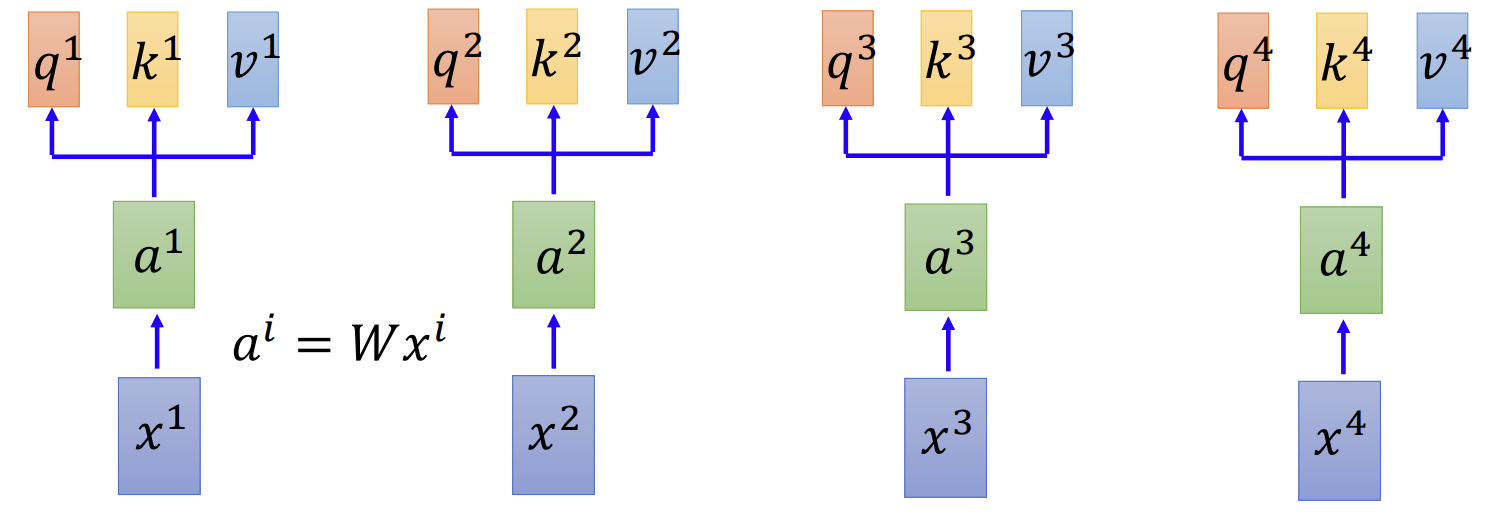
\includegraphics[width=1\textwidth]{figures/self_attention_matrix.png}
        \end{column}
        \begin{column}{0.4\textwidth}
            \begin{itemize}
                \item $q:$ query (to math others)
                \begin{align*}
                    q^i = W^{q}a^i
                \end{align*}
                \item $k:$ key (to be matched)
                \begin{align*}
                    k^i = W^{k}a^i
                \end{align*}
                \item $v:$ information to be extracted
                \begin{align*}
                    v^i = W^{v}a^i
                \end{align*}
            \end{itemize}
        \end{column}
    \end{columns}
\end{frame}

%------------------------------------------------

\begin{frame}{Image Encoder - Self Attention}
    \begin{columns}
        \begin{column}{0.6\textwidth}
            \begin{figure}
                \centering
                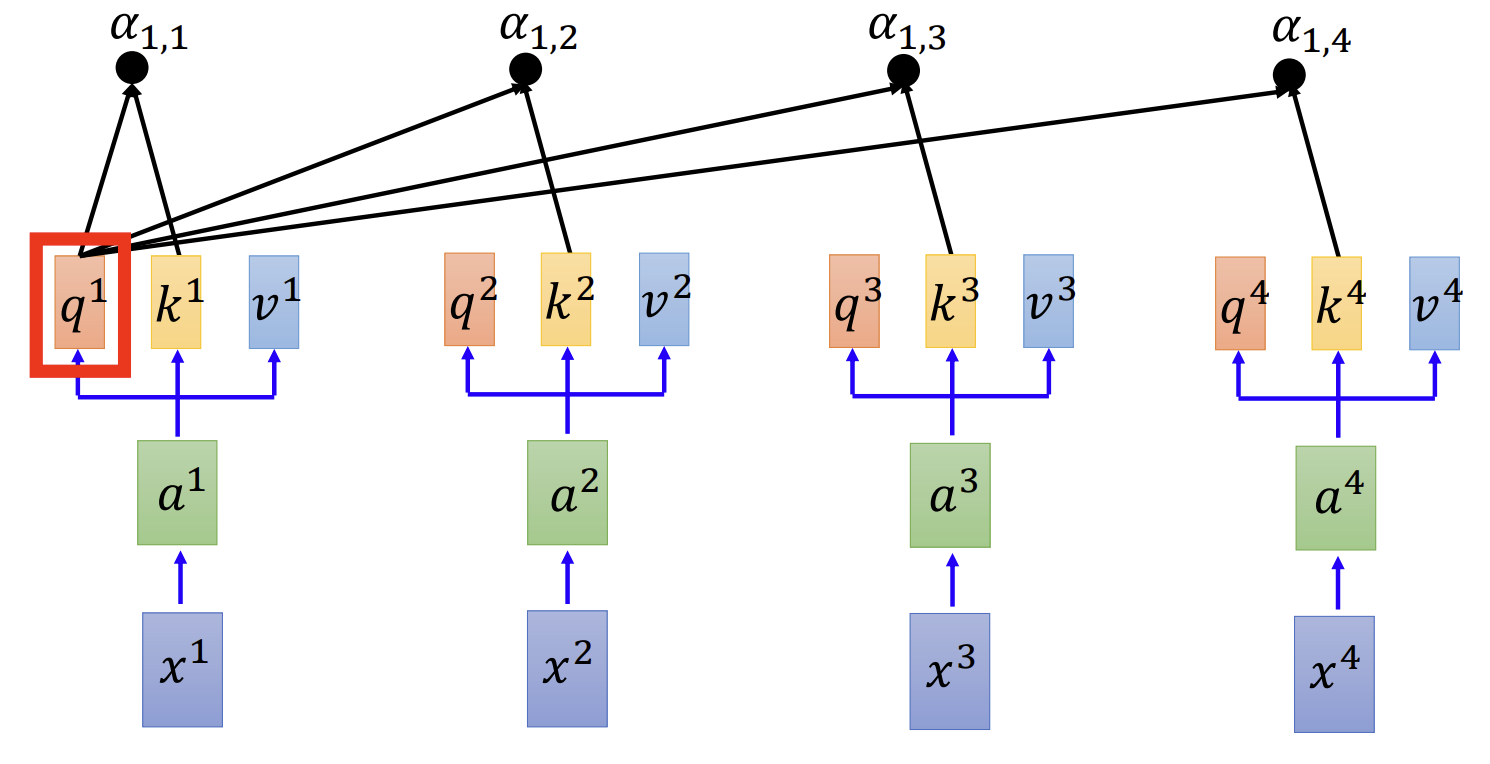
\includegraphics[width=1\linewidth]{figures/self_attention_dot_product.png}
                \label{self_attention_dot_product}
            \end{figure}
        \end{column}

        \begin{column}{0.4\textwidth}
            Use each query to compute the dot product with all keys. The formula for computing the attention weights is called Scaled Dot-Product Attention:
            \begin{align*}
                \alpha_{1,i}= q^i \cdot k^i / \sqrt{d}, d \ \text{dimension of} \ q^i, k^i
            \end{align*}  
        \end{column}
    \end{columns}
\end{frame}

%------------------------------------------------

\begin{frame}{Image Encoder - Self Attention}
    \begin{columns}
        \begin{column}{0.6\textwidth}
            \begin{figure}
                \centering
                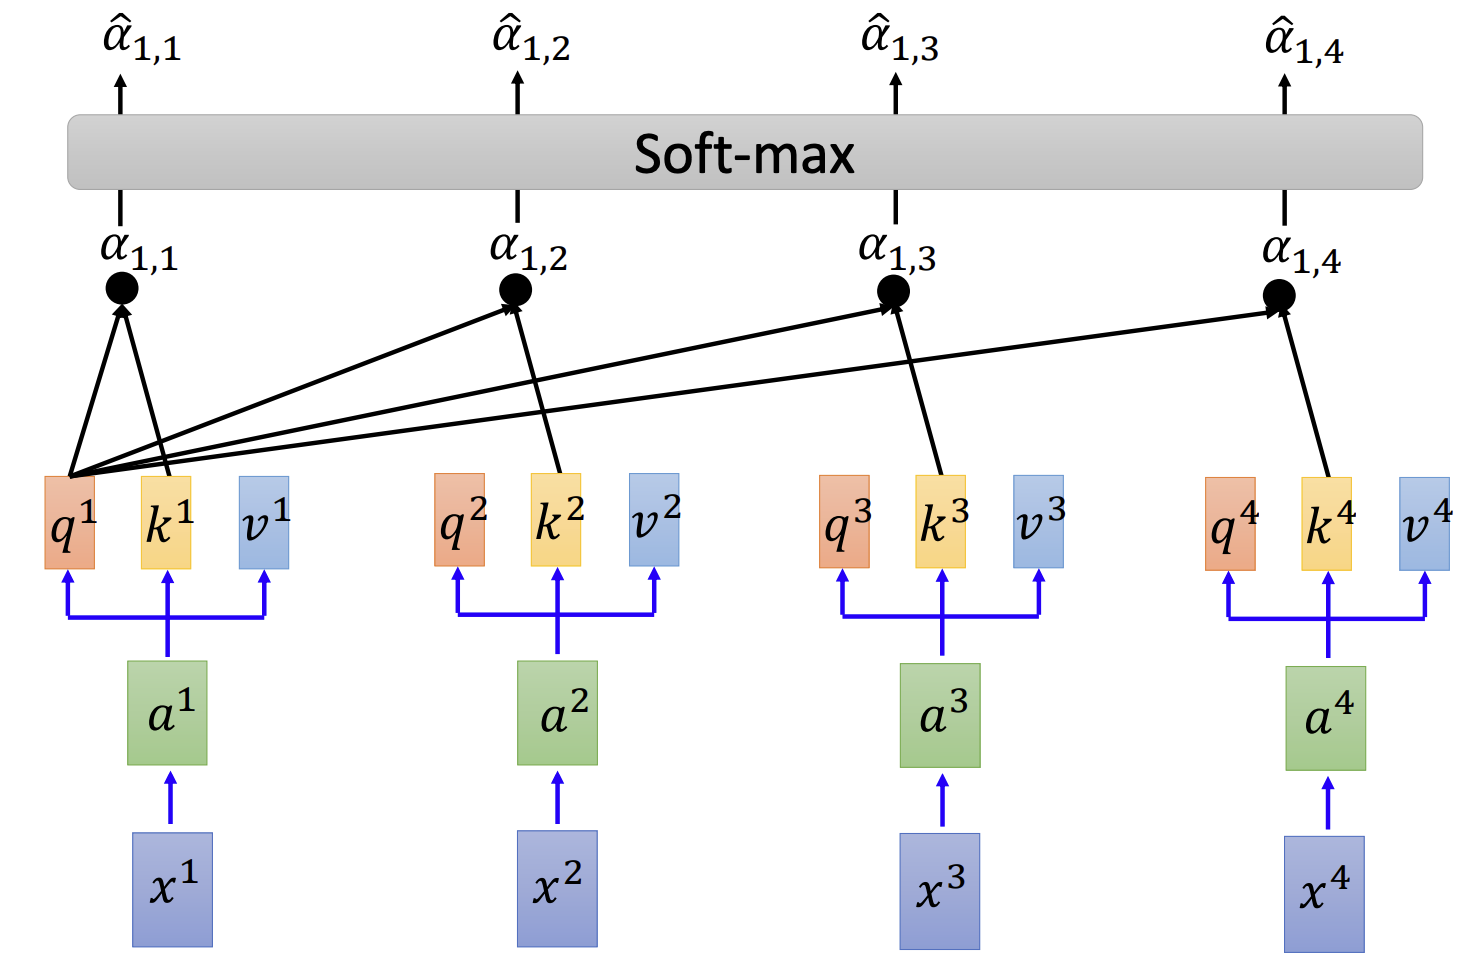
\includegraphics[width=1\linewidth]{figures/self_attention_softmax.png}
                \label{self_attention_softmax}
            \end{figure}
        \end{column}
        \begin{column}{0.4\textwidth}
            Apply a soft-max function to obtain the normalized attention weights:
            \begin{align*}
                \hat{\alpha}_{1,i}= \exp(\alpha_{1,i}) / \sum\nolimits_{j=1}^{N} \exp(\alpha_{1,j}) 
            \end{align*}
        \end{column}
    \end{columns}
\end{frame}

%------------------------------------------------

\begin{frame}{Image Encoder - Self Attention}
    \begin{columns}
        \begin{column}{0.6\textwidth}
            \begin{figure}
                \centering
                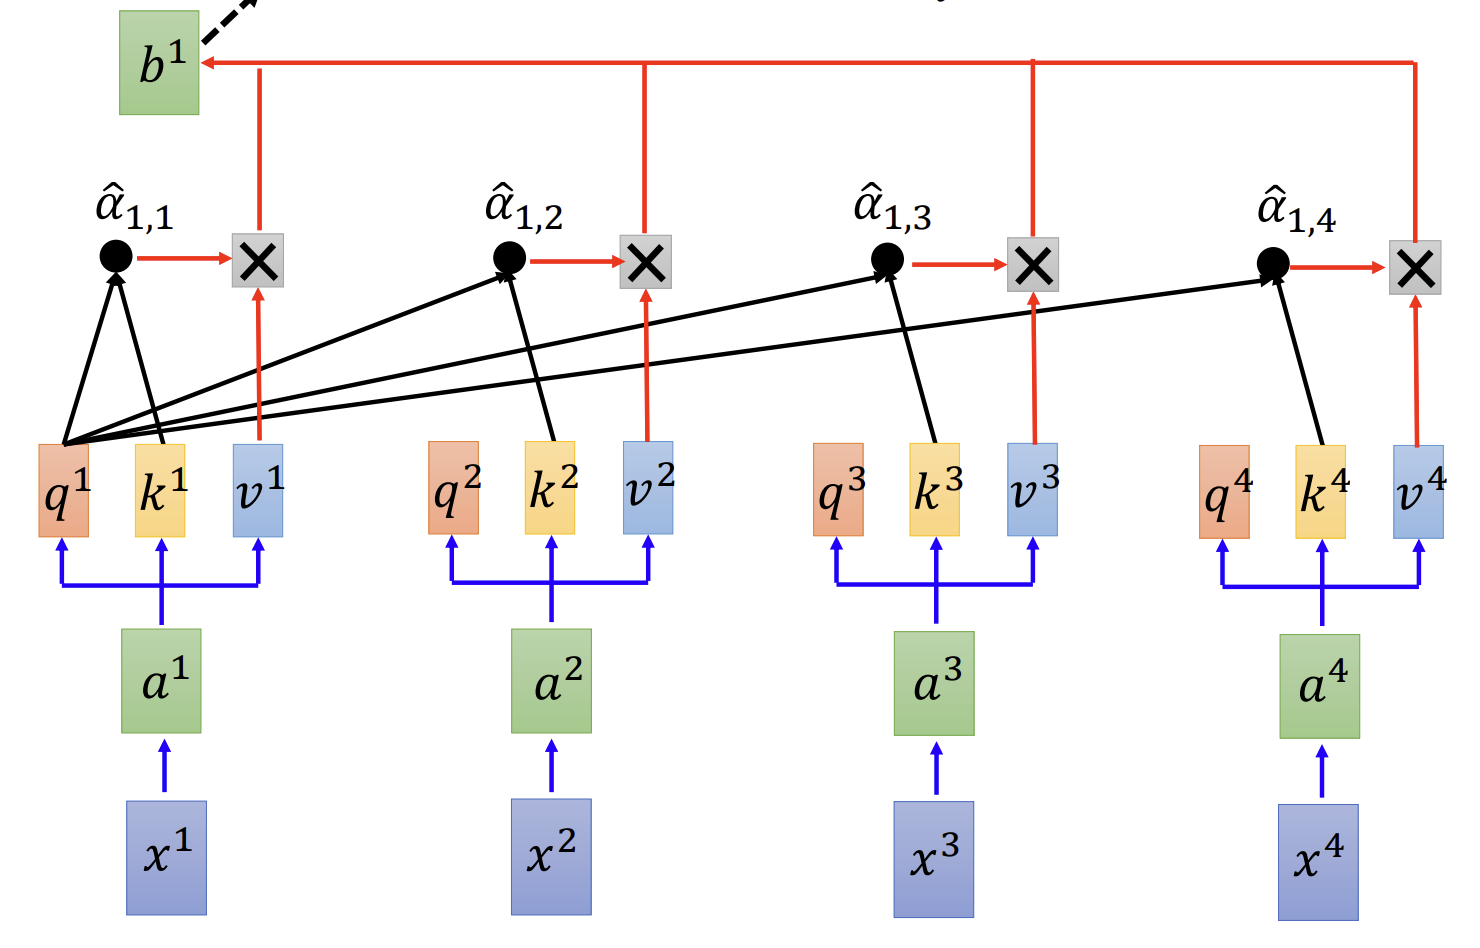
\includegraphics[width=1\linewidth]{figures/self_attention_summing.png}
                \label{self_attention_summing}
            \end{figure}
        \end{column}
        \begin{column}{0.4\textwidth}
            The output $b^i$ of the self-attention layer is the sum of the normalized attention weights and the value vectors:
            \begin{align*}
                b^1 = \sum\nolimits_{i=1}^{N} \hat{\alpha}_{1,i}v^i
            \end{align*}
        \end{column}
    \end{columns}
\end{frame}

%------------------------------------------------

\begin{frame}{Image Encoder - Self Attention conc.}
    \begin{figure}
        \centering
        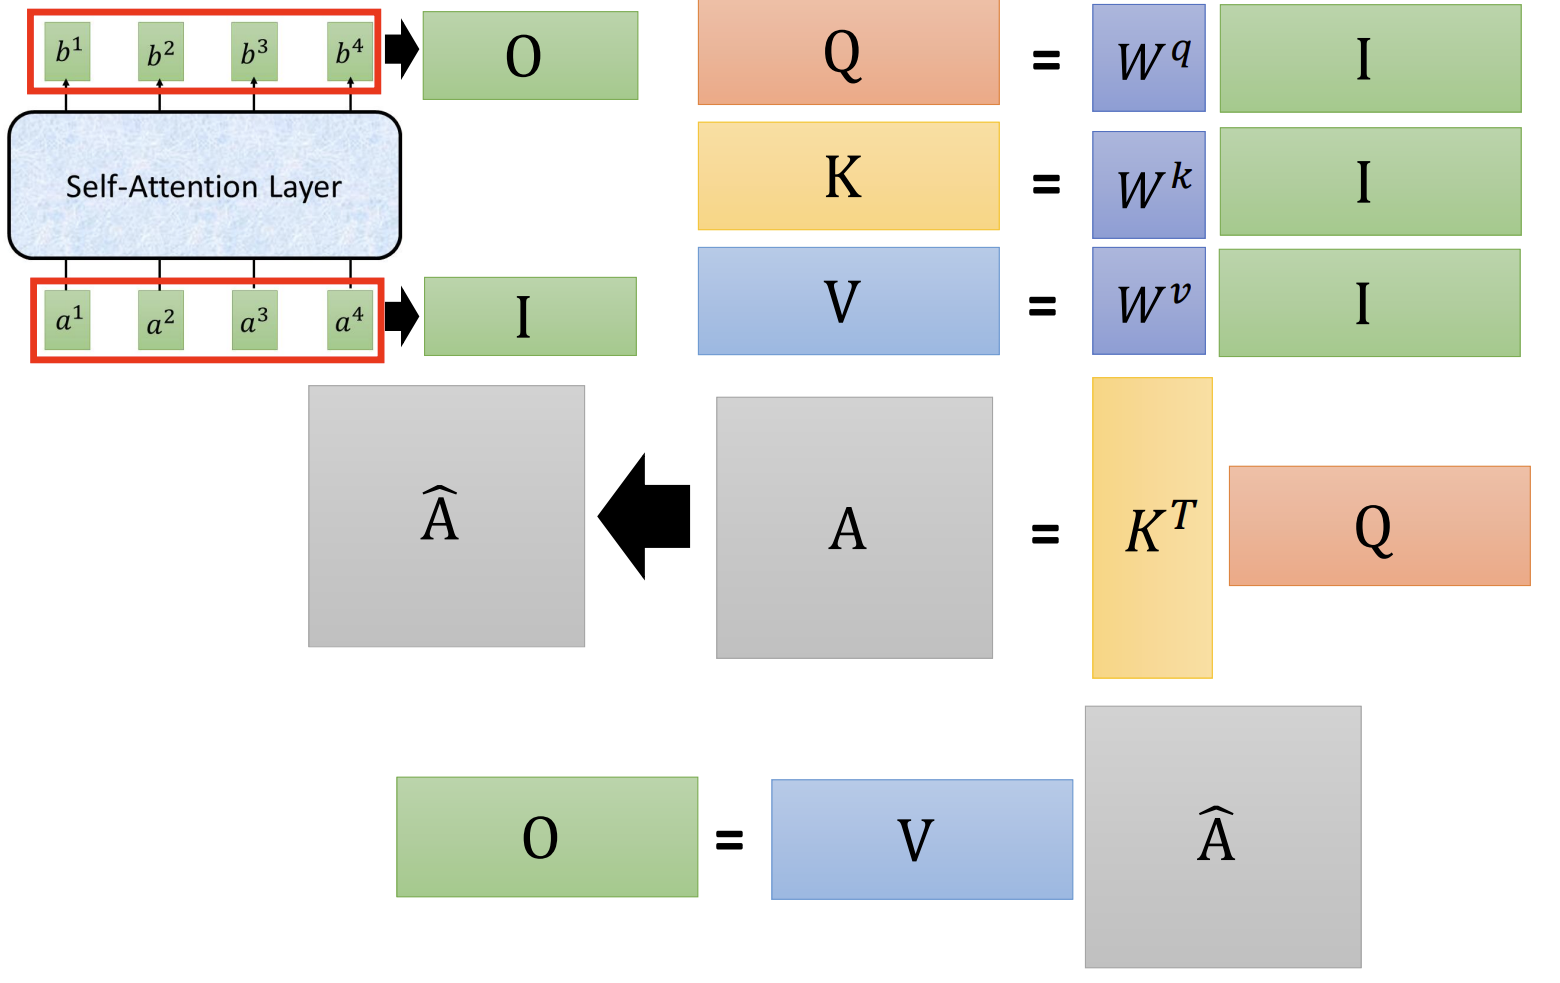
\includegraphics[width=0.6\linewidth]{figures/self_attention_matrix_multiplication.png}
        \label{self_attention_matrix_multiplication}
    \end{figure}
    All these vector operations can concatenated into matrix multiplications. Therefore, GPU can be used to accelerate the computation.\\


\end{frame}

%------------------------------------------------

\begin{frame}{Self Attention - Multihead Self Attention}
    \begin{figure}
        \centering
        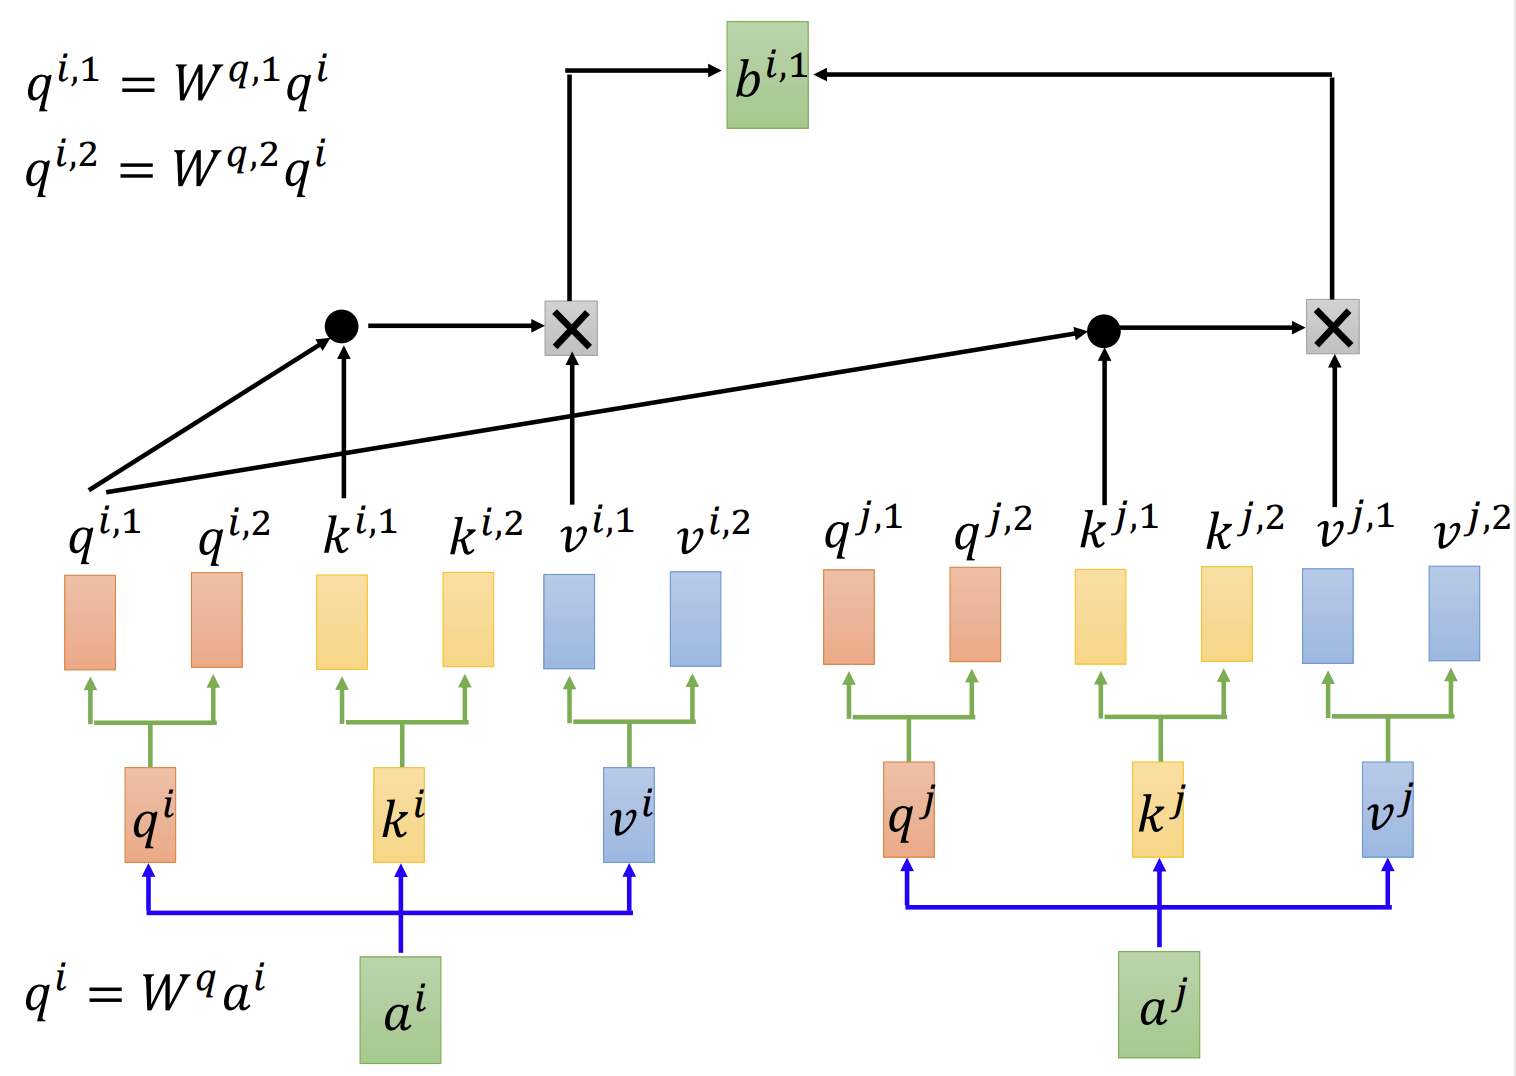
\includegraphics[width=0.6\linewidth]{figures/multihead_self_attention.png}
        \label{multihead_self_attention}
    \end{figure}
    We have more than one $W^q$, $W^k$, and $W^v$ to learn different linear projections. The output of each head is concatenated and projected to the final output dimension.
\end{frame}

%------------------------------------------------

\begin{frame}{Self Attention - Multihead Self Attention}
    \begin{figure}
        \centering
        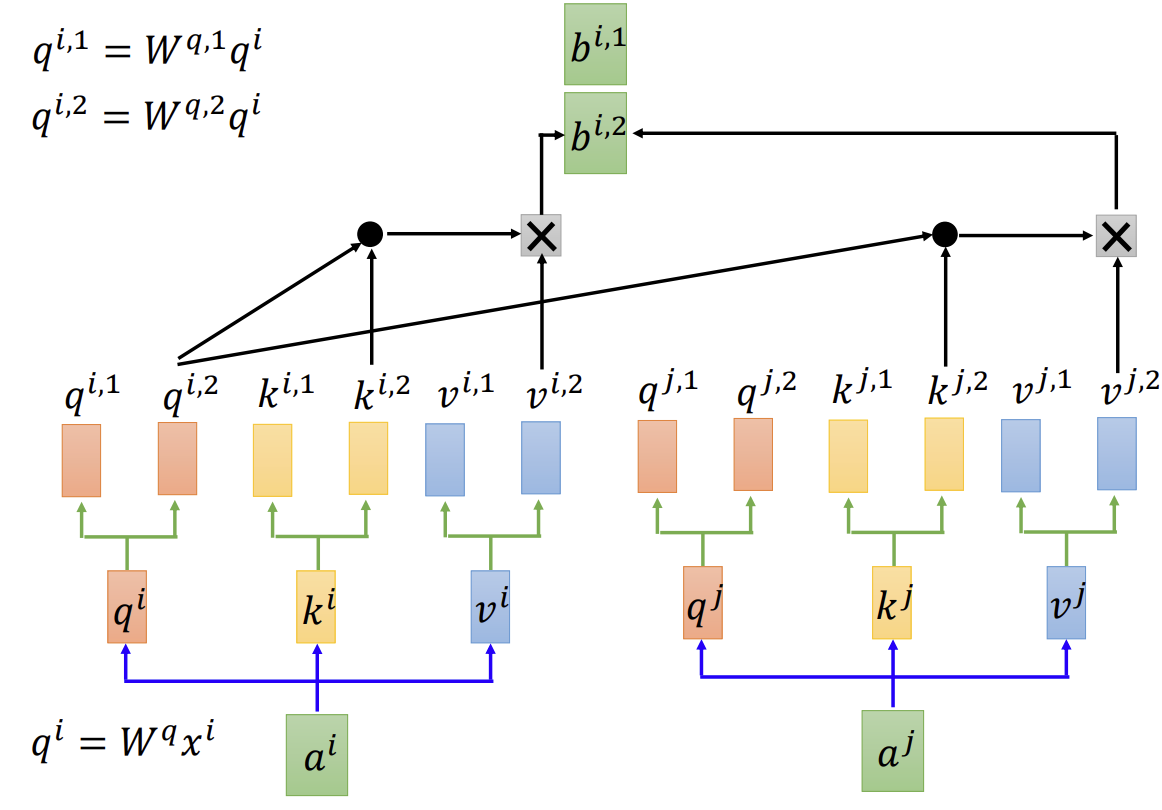
\includegraphics[width=0.6\linewidth]{figures/multihead_self_attention_weights.png}
        \label{multihead_self_attention_weights}
    \end{figure}
    The calculation of $b^{i,1}$ only includes the multiplication of $q^i$ and $k^i$ in the first head.
\end{frame}

%------------------------------------------------

\begin{frame}{Self Attention - Multihead Self Attention}
    \begin{columns}
        \begin{column}{0.7\textwidth}
            \begin{figure}
            \centering
            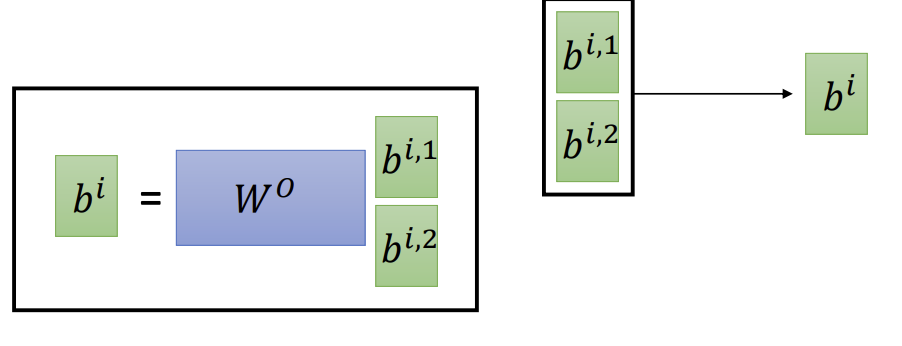
\includegraphics[width=0.9\linewidth]{figures/multihead_self_attention_output_concatenation.png}
            \label{multihead_self_attention_output_concatenation}
            \end{figure}
        \end{column}
        \begin{column}{0.3\textwidth}
            Two outputs of the multihead self-attention layer are concatenated by multiplying a $W^0$ matrix and projected to the final output dimension.
        \end{column}
    \end{columns}
\end{frame}




%------------------------------------------------

\begin{frame}{Image Encoder - Vision Transformer}
    \begin{figure}
        \centering
        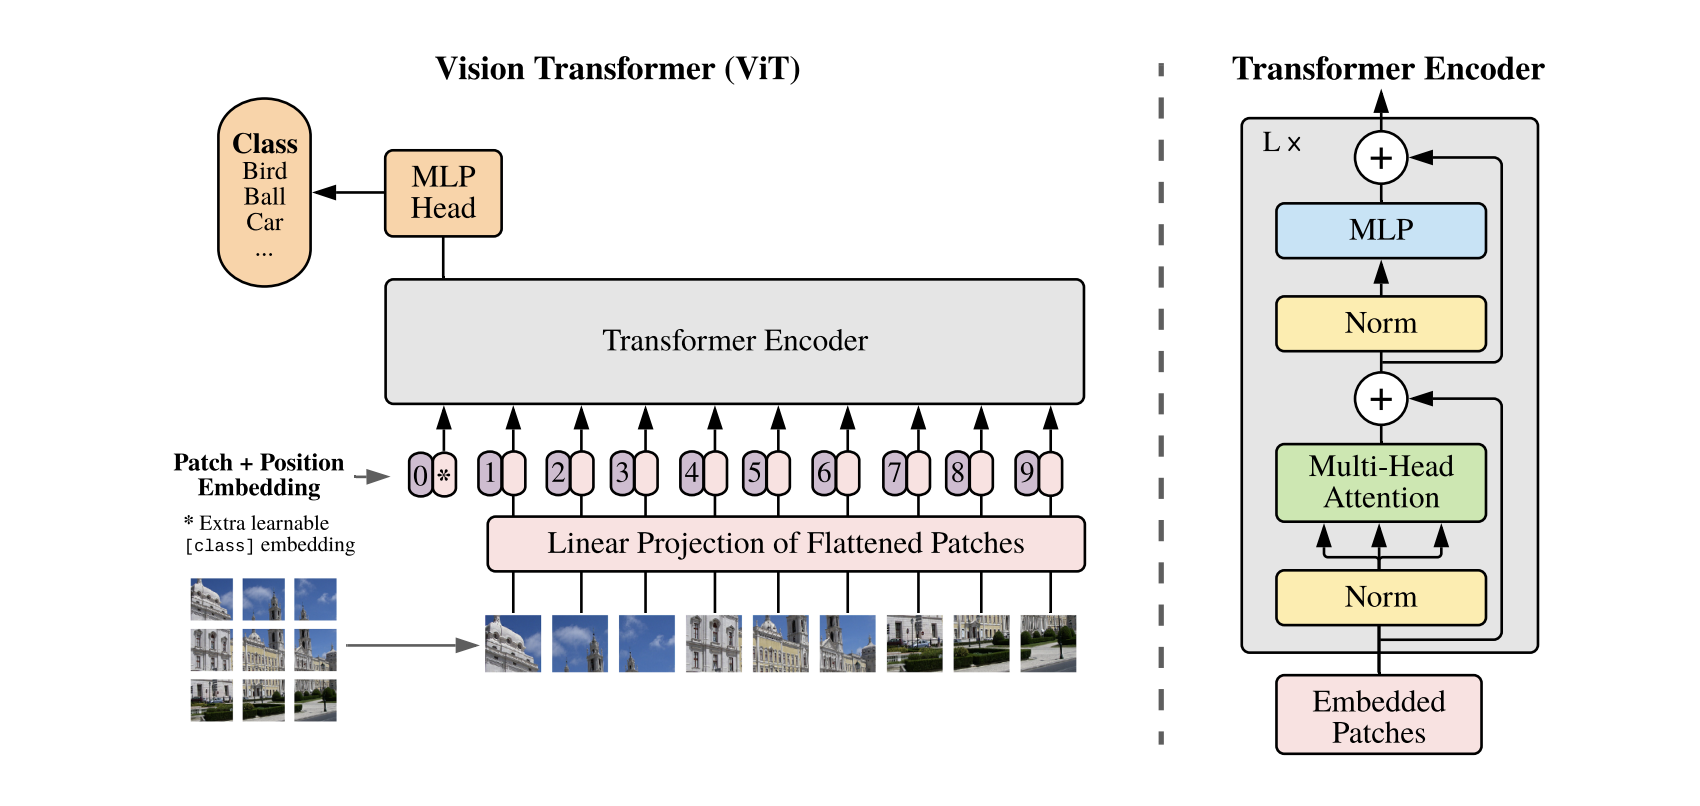
\includegraphics[width=0.9\linewidth]{figures/ViT_architecture.png}
        \label{ViT_architecture}
    \end{figure}
\end{frame}

%------------------------------------------------
\subsection{Text Encoder}
%------------------------------------------------

\begin{frame}{Text Encoder - Modified Transformer}
    \begin{block}{Quote}
        \textit{As a base size we use a 12-layer 512-wide model with 8 attention heads. The transformer operates on a \textbf{lower-cased byte pair encoding (BPE) representation} of the text (Sennrich et al., 2015). The text sequence is bracketed
        with [SOS] and [EOS] tokens and the activations of the highest layer of the transformer at the [EOS] token are used as the feature representation of the text which is layer normalized and then linearly projected into the multi-modal embedding space. Masked self-attention was used in the text encoder to preserve the ability to add language modeling as an auxiliary objective, though exploration of this is left as
        future work.}
        
    \end{block}
    
    
\end{frame}

%------------------------------------------------



\begin{frame}{Subword-based Tokenization - BPE}
    \textbf{Byte-Pair Encoding (BPE)}
    is a simple form of data compression algorithm in which the most common pair of consecutive bytes of data is replaced with a byte that does not occur in that data.
    \medskip
    \begin{block}{Motivation}
        Transformer has limited capacity to process long sequences, BPE is used to reduce the vocabulary size and the length of the input sequence
    \end{block}
    \medskip
    \textbf{$[SOS] $ and $[EOS]$} special tokens added to the beginning and end of the text, indicating the start and end of the text.
    
\end{frame}

%------------------------------------------------

\begin{frame}{Subword-based Tokenization - BPE}
    
    \begin{figure}
        \centering
        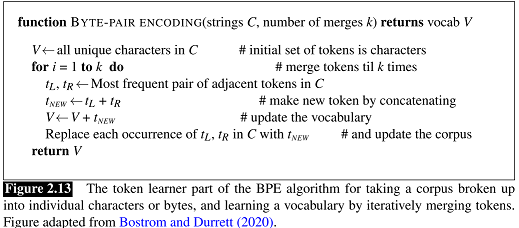
\includegraphics[width=0.9\linewidth]{figures/BPE.png}
        \label{BPE_example}
    \end{figure}
    
\end{frame}

%------------------------------------------------


\begin{frame}{BPE - example}
    \begin{figure}
        \centering
        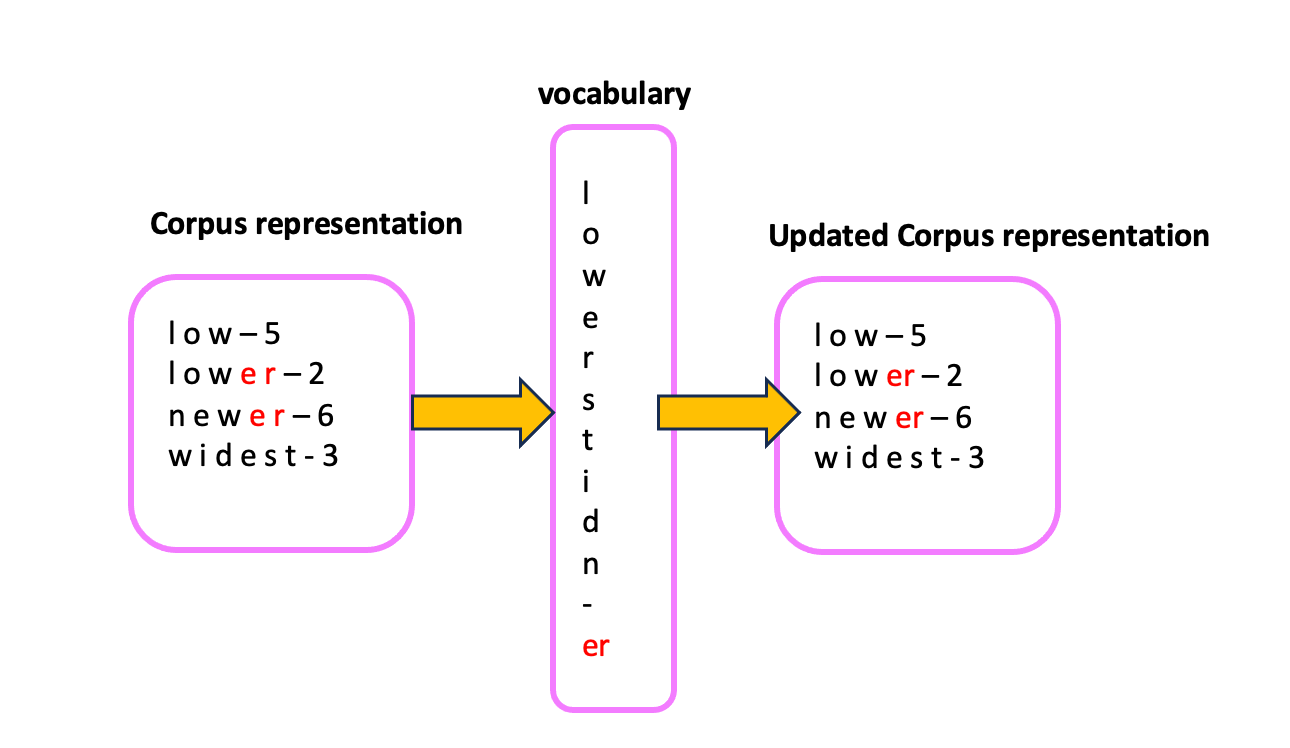
\includegraphics[width=0.9\linewidth]{figures/BPE_demo.png}
        \label{BPE_demo}
    \end{figure}
\end{frame}

%------------------------------------------------

\begin{frame}{Encoder}
    \begin{figure}
        \centering
        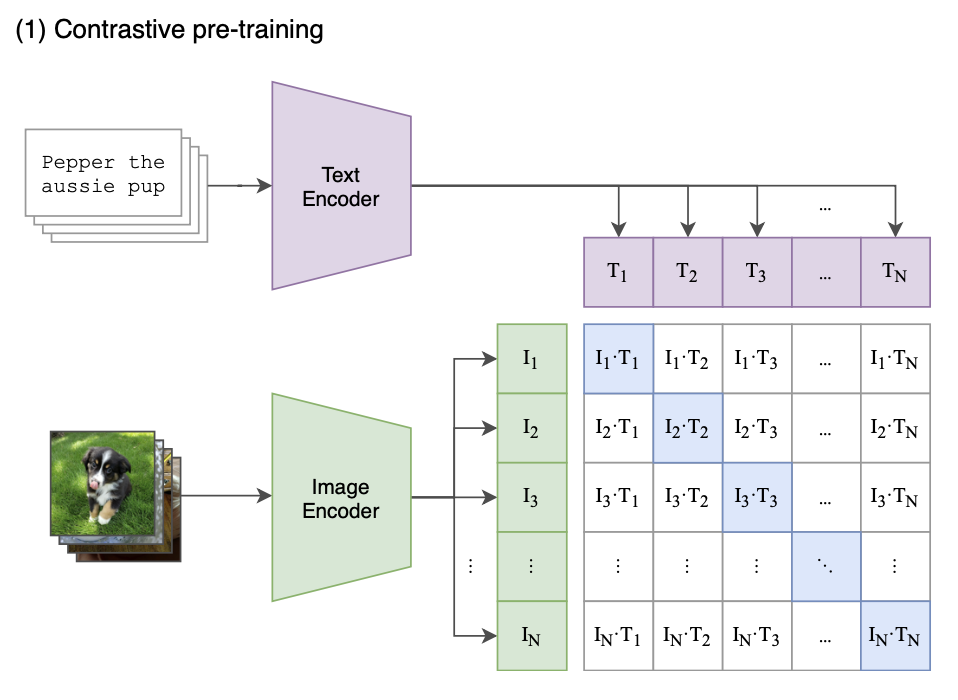
\includegraphics[width=0.7 \linewidth]{figures/contrastive_pre_training.png}
    \end{figure}
\end{frame}

%------------------------------------------------
\section{Training}
%------------------------------------------------

\begin{frame}{Training}
    Both models are optimized during pretraining to align similar text ad images in vector space. It does this by taking image-text pairs and pushing their output vectors nearer in vector space while pushing the output vectors of dissimilar pairs further apart.
\end{frame}

%------------------------------------------------

\begin{frame}{Pre-Training Method Selection-Distance Metric Learning}
    \begin{block}{Contrastive loss}
    takes pairs of example as input and trains a network to predict whether two inputs are from the same class or not.
     \begin{align*}
        \mathcal{L}_{\text {cont }}^m\left(x_i, x_j ; f\right)=\mathbf{1}\left\{y_i=y_j\right\}\left\|f_i-f_j\right\|_2^2+\mathbf{1}\left\{y_i \neq y_j\right\} \max \left(0, m-\left\|f_i-f_j\right\|_2\right)^2
    \end{align*}
    \end{block}
    \bigskip
    $1\{y_i=y_j\}$ indicator function
    ,
    $\left\|f_i-f_j\right\|_2 = \sqrt{\sum_k(f_i^{(k)}-f_j^{(k)})^2}$ \\
    \medskip
    $\max \left(0, m-\left\|f_i-f_j\right\|_2\right)^2$ 
    \begin{itemize}
        \item if $m-\left\|f_i-f_j\right\|_2^2  \leq 0 =0$ no loss is added\\
        \item elif $m-\left\|f_i-f_j\right\|_2^2  > 0 =0$ the loss is positive, penalty added, separating two embeddings in Euclidean space
    \end{itemize}
    
\end{frame}

%------------------------------------------------

\begin{frame}{Pretraining Method Selection-Distance Metric Learning}
    \begin{block}{Triplet loss}
    composed of triplets, consisting of a query, a positive example, and a negative example
        \begin{align*}
        \mathcal{L}_{\text {tri }}^m\left(x, x^{+}, x^{-} ; f\right)=\max \left(0,\left\|f-f^{+}\right\|_2^2-\left\|f-f^{-}\right\|_2^2+m\right)
        \end{align*}
     \end{block}
    \bigskip
    $\max \left(0,\left\|f-f^{+}\right\|_2^2-\left\|f-f^{-}\right\|_2^2+m\right)$ 
    \begin{itemize}
        \item if $\left\|f-f^{-}\right\|_2^2 - \left\|f-f^{+}\right\|_2^2 \geq m$ no loss is added\\
        \item elif $\left\|f-f^{-}\right\|_2^2 - \left\|f-f^{+}\right\|_2^2 < m$ the loss is positive, model penalised
    \end{itemize}
    
\end{frame}

%------------------------------------------------

\begin{frame}{Pretraining Method Selection-Distance Metric Learning}
    \textbf{Limitation} both loss functions are known to suffer from slow convergence and they often require expensive data sampling method to provide nontrivial pairs or triplets to accelerate the training\\
    Trivial pairs $\rightarrow$ weak gradient updates $\rightarrow$ slow convergence\\
    \bigskip
    Nontrivial pairs
    \begin{itemize}
        \item Hard positive pairs: Pairs from the same class that are far apart in feature space force the model to learn better embeddings to bring them closer.
        \item Hard negative pairs: Pairs from different classes that are close together push the model to better separate different classes.
    \end{itemize}
\end{frame}

%------------------------------------------------

\begin{frame}{Pre-Training Method Selection-Distance Metric Learning with Multiple Negative Examples}
    \textbf{Goal} 
    \begin{itemize}
        \item positives examples $\rightarrow$ shorten distances between embedding vectors 
        \item negative examples $\rightarrow$ enlarging distances
    \end{itemize}
    \bigskip
    \textbf{Problem}\\
    During the update, the triplet loss only compares an example with one negative example while ignoring negative examples from the rest of the classes. The consequence is the embedding vector of an example is only guaranteed to be far from the selected negative class but not the others. \\
    \bigskip
    \textbf{Solution} A loss function that recruits multiple negatives for each update
    
\end{frame}

%------------------------------------------------

\begin{frame}{Pretraining Method Selection - Distance Metric Learning with Multiple Negative Examples}
    \begin{figure}
        \centering
        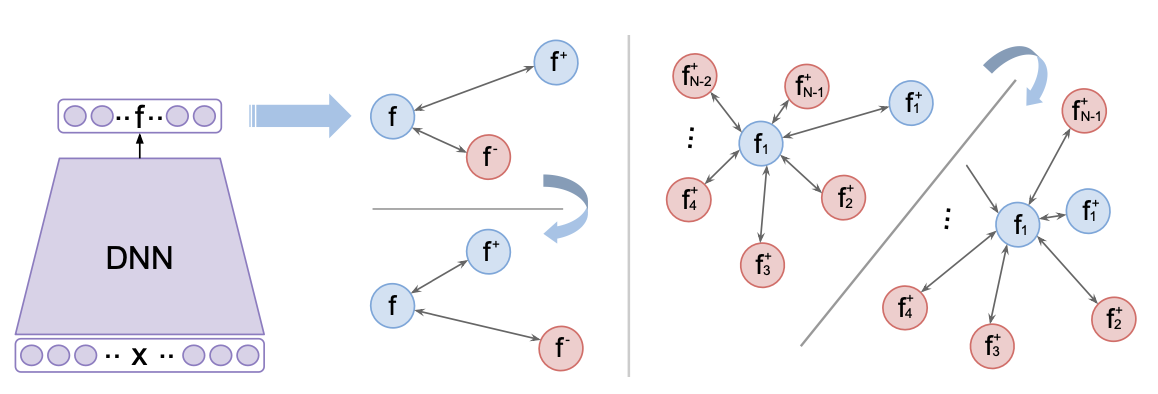
\includegraphics[width=0.9\linewidth]{figures/one_negative_vs_multiple_negative.png}
        \caption{Triplet Loss vs. Multiple Negative Examples Loss }
        \label{onmn}
    \end{figure}
\end{frame}

%------------------------------------------------

\begin{frame}{Pretraining Method Selection-Distance Metric Learning with Multiple Negative Examples}
    \begin{block}{(N+1)-tuplet loss}
    \begin{align*}
        \mathcal{L}\left(\left\{x, x^{+},\left\{x_i\right\}_{i=1}^{N-1}\right\} ; f\right)=\log \left(1+\sum_{i=1}^{N-1} \exp \left(f^{\top} f_i-f^{\top} f^{+}\right)\right)
    \end{align*}
    \end{block}
    \bigskip
    Cosine similarity $f^Tf_i=\left||f\right||\left||f_i\right||\cos{\theta}$\\
    \begin{itemize}
        \item if dot product is large, $\cos{\theta} \rightarrow 1$, $\theta \rightarrow 0$, high similarity
        \item small, $\cos{\theta} \rightarrow 0$, $\theta \rightarrow \perp$, no similarity
        \item negative, $\cos{\theta} \rightarrow -1$, $\theta \rightarrow 180\degree$, strong dissimilarity
    \end{itemize}
\end{frame}

%------------------------------------------------

\begin{frame}{Pretraining Method Selection- N-pair Loss Batch Construction}
    \textbf{Problem} When the batch size of Stochastic Gradient Descent is $M$, there are $M \times (N+1)$ examples to be passed through $f$ at one update. Too large and impractical to scale.\\
    \bigskip
    \textbf{Effective Batch Construction}\\
    \medskip
    $N$ pairs of examples from $N$ different classes $\left\{\left(x_1, x_1^{+}\right), \cdots,\left(x_N, x_N^{+}\right)\right\}$\\
    \medskip
    Build $N$ tuples, denoted as $\left\{S_i\right\}_{i=1}^N$, from the $N$ pairs.
    \medskip
    \begin{itemize}
        \item $S_i=\left\{x_i, x_1^{+}, x_2^{+}, \cdots, x_N^{+}\right\}$
        \smallskip
        \begin{itemize}
            \item $x_i$ is the query for $S_i$ 
            \smallskip
            \item $x_i^+$ a positive example, rest are negative examples
        \end{itemize}
    \end{itemize}
\end{frame}

%------------------------------------------------

\begin{frame}{Pretraining Method Selection-Distance Metric Learning with Multiple Negative Examples}
    \begin{figure}
        \centering
        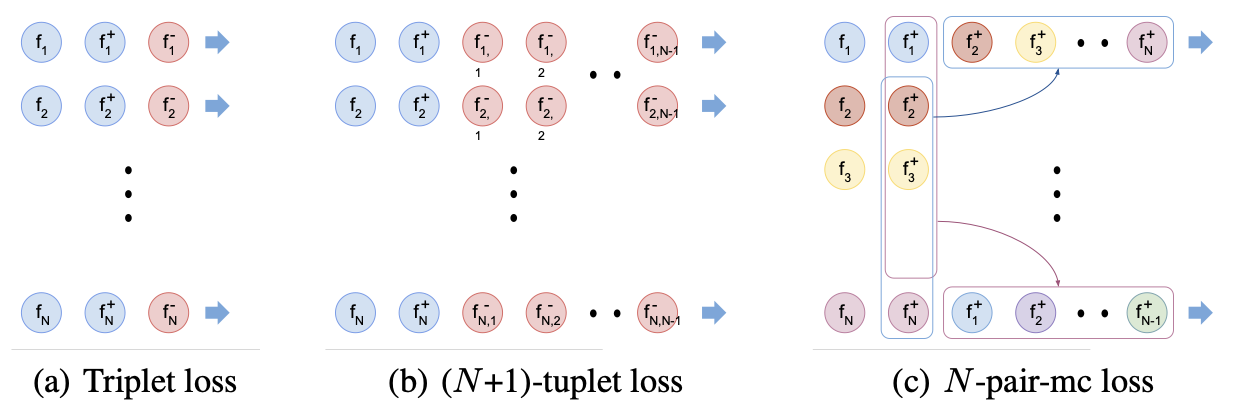
\includegraphics[width=0.9\linewidth]{figures/pushing_N_examples_simultaneously.png}
        \label{n_examples}
    \end{figure}
\end{frame}

%------------------------------------------------

\begin{frame}{Pretraining Method Selection-CLIP \& Multi-class N-pair Loss}    
    \begin{figure}
        \centering
        \subfloat{{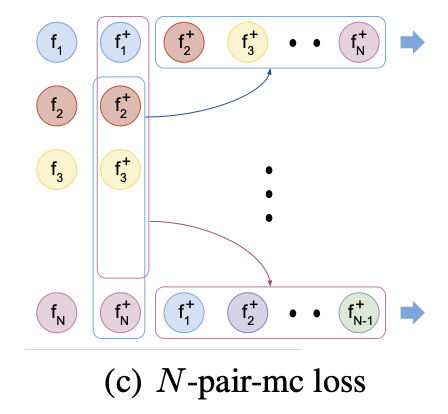
\includegraphics[width=5cm]{figures/n_pair_mc_loss.png} }}%
        \qquad
        \subfloat{{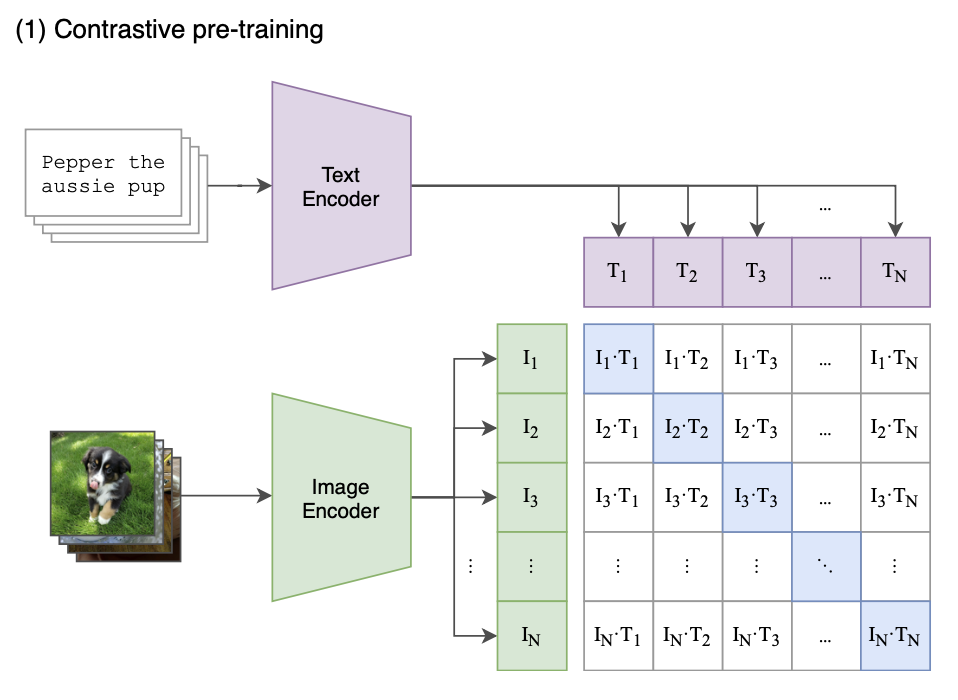
\includegraphics[width=7.5cm]{figures/contrastive_pre_training.png} }}%
    \end{figure}
\end{frame}

%------------------------------------------------

\begin{frame}{Pretraining Method Selection - Symmetric Entropy Loss(N-pair Loss/InfoNCE)}
Samples a batch of $N$ input pairs $(x_v,x_u)$ for training data, and calculate their representation pairs $(v,u)$, $i$-th pair denoted as $(v_i,u_i)$. The training objective of CLIP involves two loss functions. The first loss function is an image-text contrastive loss for the $i$-th pair: \\
    \begin{align*}
        \ell_i^{(v \rightarrow u)}=-\log \frac{\exp \left(\left\langle\mathbf{v}_i, \mathbf{u}_i\right\rangle / \tau\right)}{\sum_{k=1}^N \exp \left(\left\langle\mathbf{v}_i, \mathbf{u}_k\right\rangle / \tau\right)}\\
    \end{align*}
where $\langle v_i, u_i \rangle$ represents the cosine similarity \\
$\tau \in \mathbb{R^+}$ represents a temperature parameter, affects the smoothness of the probability distribution over the negative examples.\\

\end{frame}

%------------------------------------------------

\begin{frame}{Contrastive learning - temperature $\tau$}
    \begin{columns}
        \begin{column}{0.6\textwidth}
            \begin{figure}
                \centering
                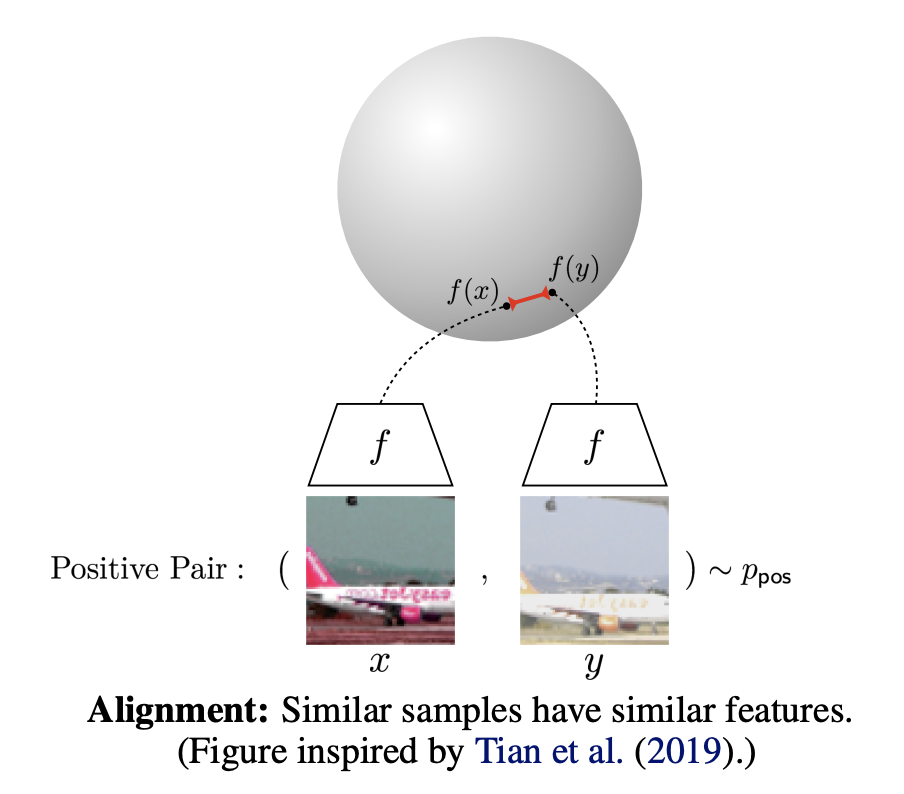
\includegraphics[width=0.85\linewidth]{figures/alignment.png}
                \label{alignment} 
            \end{figure}
        \end{column}
        \begin{column}{0.3\textwidth}
            Alignment favors encoders that assign similar features to similar samples.\\
        \end{column}
    \end{columns}
\end{frame}

%------------------------------------------------

\begin{frame}{Contrastive learning - temperature $\tau$}
    \begin{columns}
        \begin{column}{0.6\textwidth}
            \begin{figure}
                \centering
                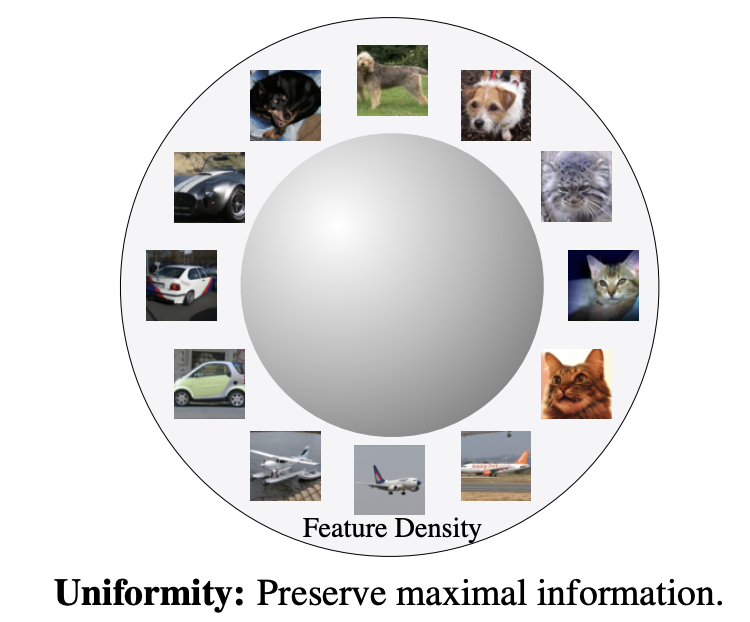
\includegraphics[width=0.8\linewidth]{figures/uniformity.png}
                \label{alignment} 
            \end{figure}
        \end{column}
        \begin{column}{0.3\textwidth}
            Uniformity prefers a feature distribution that preserves maximal information, i.e., the uniform distribution on the unit hypersphere.\\
        \end{column}
    \end{columns}
\end{frame}

%------------------------------------------------

\begin{frame}{Contrastive learning - temperature $\tau$}
    \begin{columns}
        \begin{column}{0.6\textwidth}
            \begin{figure}
                \centering
                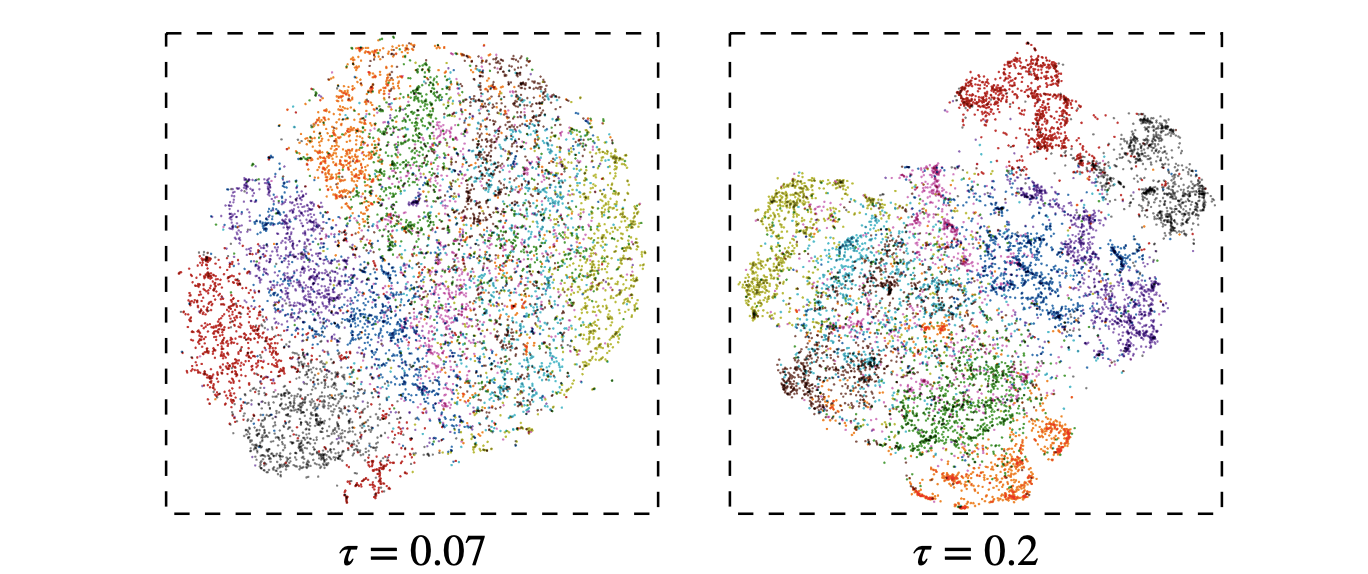
\includegraphics[width=1.1\linewidth]{figures/visualization _embedding_distribution.png}
                \label{visualization_embedding_distribution} 
            \end{figure}
        \end{column}
        \begin{column}{0.3\textwidth}
            Small temperature tends to generate
            more uniform distribution and be less tolerant to similar samples.
        \end{column}
    \end{columns}
\end{frame}

%------------------------------------------------

\begin{frame}{Pre-Training Method Selection - Symmetric Entropy Loss}
Image-to-text contrastive loss is asymmetric for each input modality. Therefore, defined a similar text-to-image contrastive loss as: \\
    \begin{align*}
        \ell_i^{(u \rightarrow v)}=-\log \frac{\exp \left(\left\langle\mathbf{u}_i, \mathbf{v}_i\right\rangle / \tau\right)}{\sum_{k=1}^N \exp \left(\left\langle\mathbf{u}_i, \mathbf{v}_k\right\rangle / \tau\right)} \\
    \end{align*}
Final training loss is then computed as a weighted combination of the two losses averaged over all positive image-text pairs in each batch:\\
    \begin{align*}
        \mathcal{L}=\frac{1}{N} \sum_{i=1}^N\left(\lambda \ell_i^{(v \rightarrow u)}+(1-\lambda) \ell_i^{(u \rightarrow v)}\right)
    \end{align*}
\end{frame}

%------------------------------------------------


\begin{frame}{Analysis - Initial Comparison to Visual N-Grams }
    \begin{figure}
        \centering
        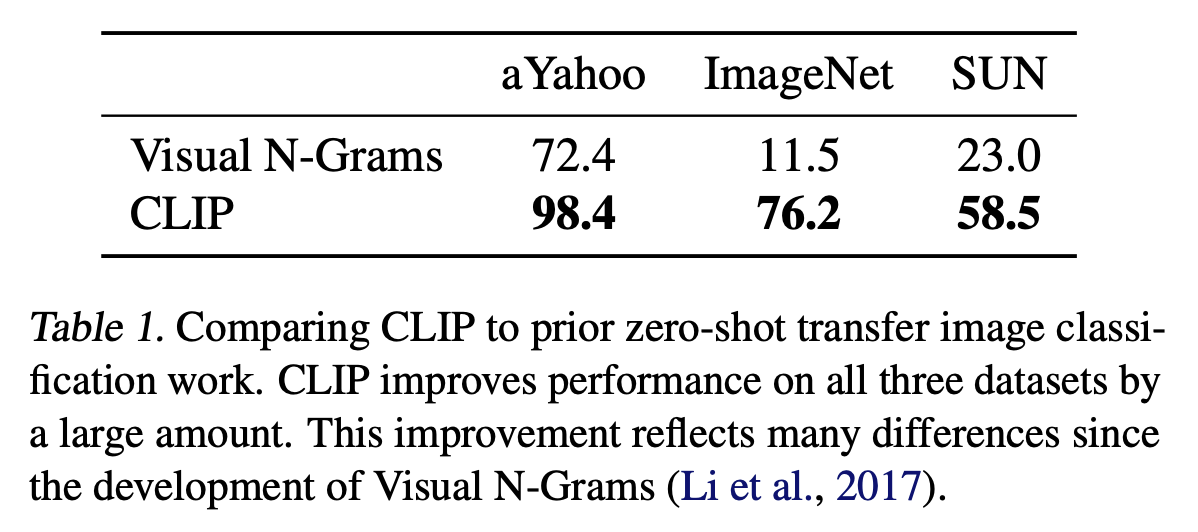
\includegraphics[width=0.55\linewidth]{figures/comparison_visual_n_grams .png}
    \end{figure}
    \begin{itemize}
        \item matches the performance of the original ResNet50 despite using one of the 1.28 million crowd-labeled training examples
        \item high 95\% top-5 accuracy
            \begin{itemize}
                \item any of the model 5 highest probability answers must match the expected answer
            \end{itemize}
        \item Differences controlled comparison between CLIP ResNtt50 and N-Grams on the same YFCC100M dataset, matched performance
    \end{itemize}

\end{frame}

%------------------------------------------------

\begin{frame}{Analysis - Zero-Shot Performance}
\begin{columns}
    \begin{column}{0.48\textwidth}
    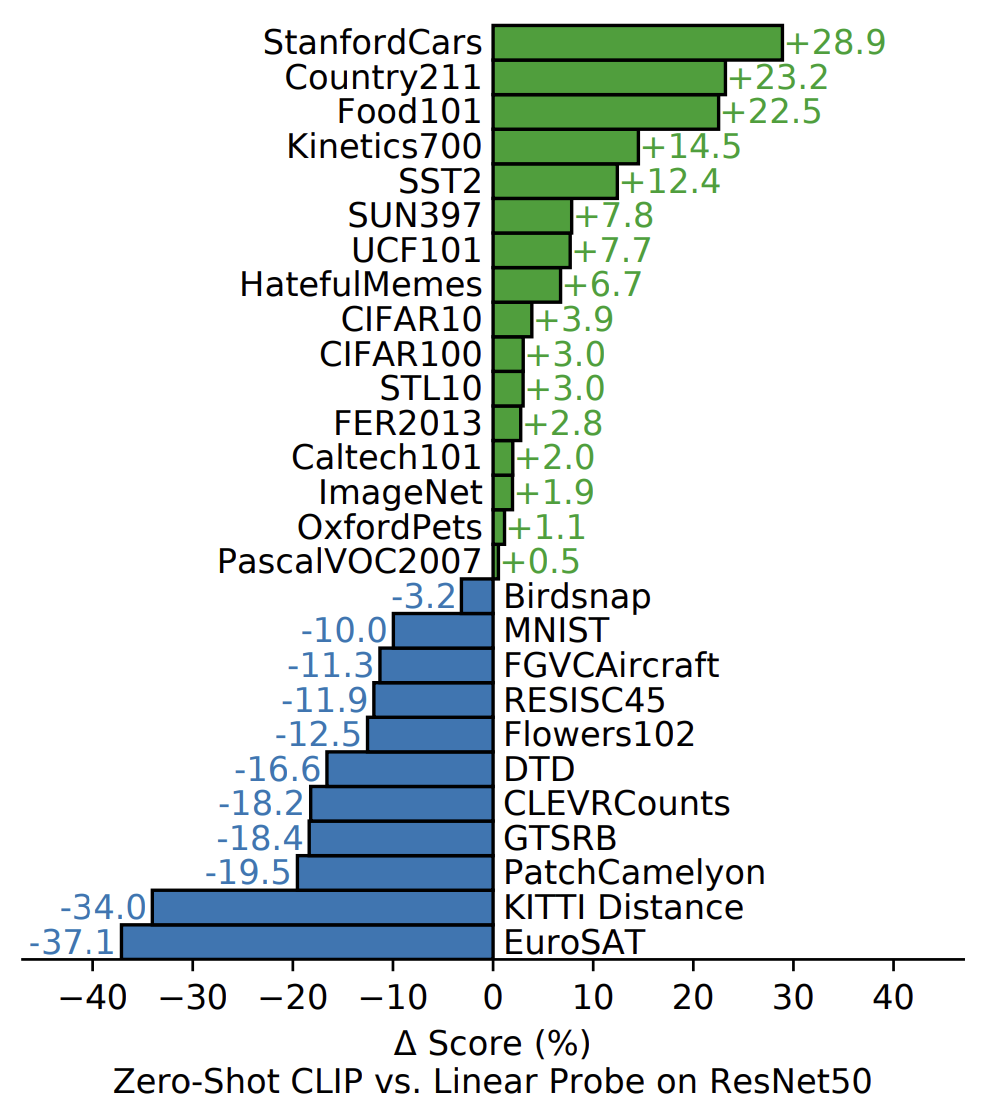
\includegraphics[width=\textwidth]{figures/zero_shot_fully_supervised_baseline.png}
    \end{column}

    \begin{column}{0.5\textwidth}
        \textbf{Comparison}\\
        \begin{itemize}
            \item \textbf{baseline} a fully supervised, regularized, logistic regression classifier on the features of the canonical ResNet50 across 27 datasets
        \end{itemize}
        \textbf{Outperforms}\\
        \begin{itemize}
            \item limited number of labeled examples
            \item general object classification datasets
            \item datasets measuring action recognition in videos
        \end{itemize}
        \textbf{Underperforms}\\
        \begin{itemize}
            \item visual concepts involving verbs
            \item specialized, complex, or abstract tasks
        \end{itemize}
\end{column}
\end{columns}
\end{frame}

%------------------------------------------------

\begin{frame}{Analysis - Zero-Shot Performance}
\begin{columns}
    \begin{column}{0.45\textwidth}
    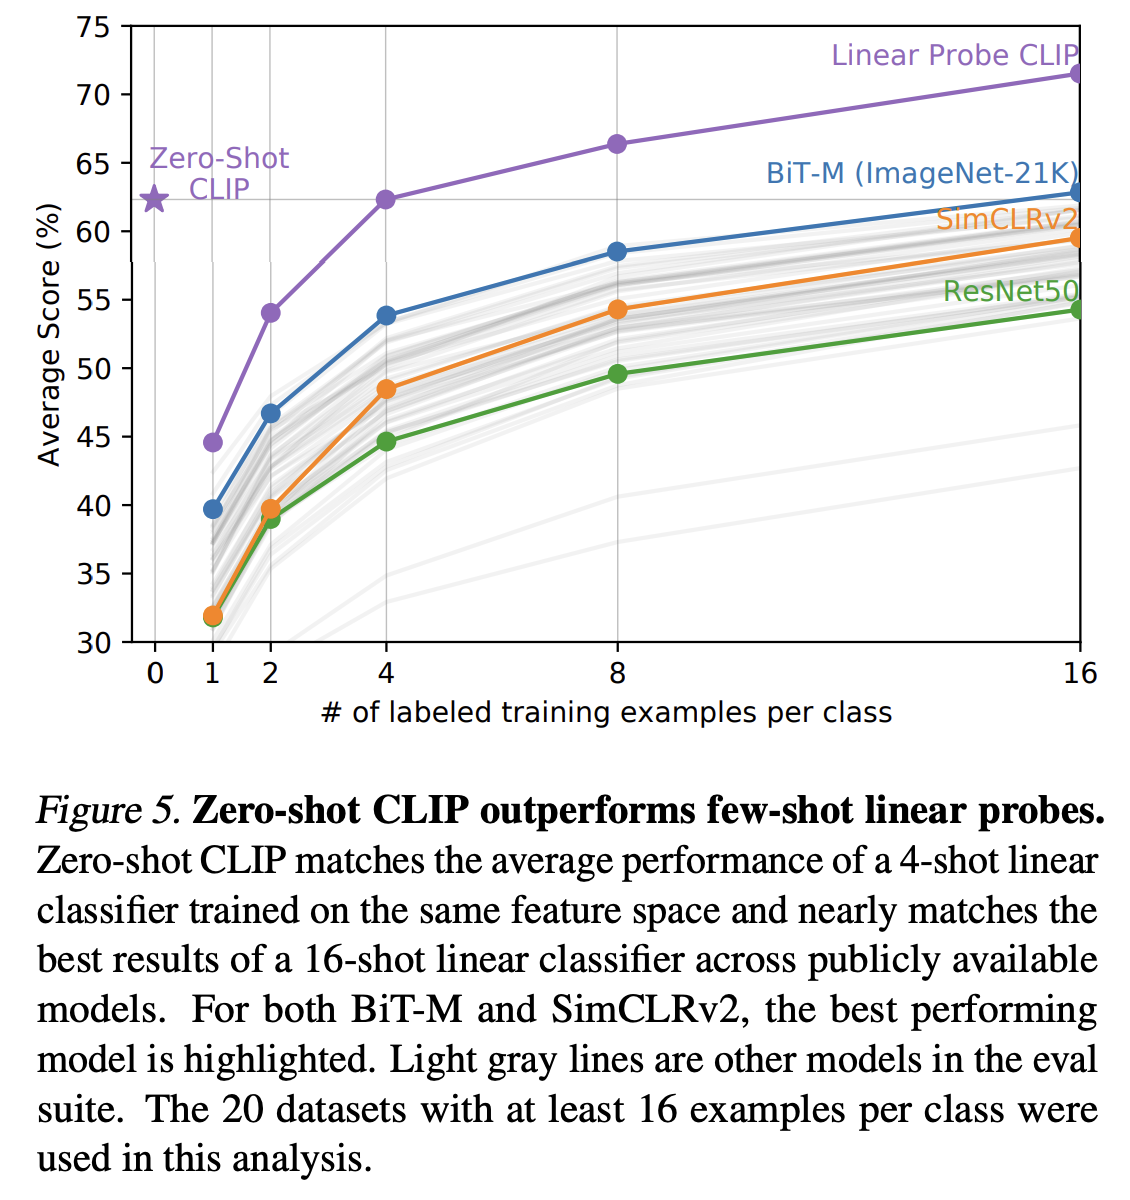
\includegraphics[width=\textwidth]{figures/few_shot_comparison.png}
    \end{column}

    \begin{column}{0.5\textwidth}
        \textbf{Comparison with few-shot methods}\\
        \begin{itemize}
            \item few-shot logistic regression on the features of many image models
        \end{itemize}
        \textbf{matches}\\
        \begin{itemize}
            \item 4-shot logistic regression on the same feature space \\
            \begin{itemize}
                \item CLIP’s zero-shot classifier:is generated via natural languags which allows for visual concepts to be directly specified
                \item normal supervised learning: must infer concepts indirectly from training examples
            \end{itemize}
        \end{itemize}
        \textbf{roughly matches}\\
        \begin{itemize}
            \item 16-shot classifier, which uses the features of a BiT-M ResNet152x2 trained on ImageNet-21K.
        \end{itemize}
\end{column}
\end{columns}
\end{frame}

%------------------------------------------------

\begin{frame}{Analysis - Representation Learning}
    \begin{figure}
        \centering
        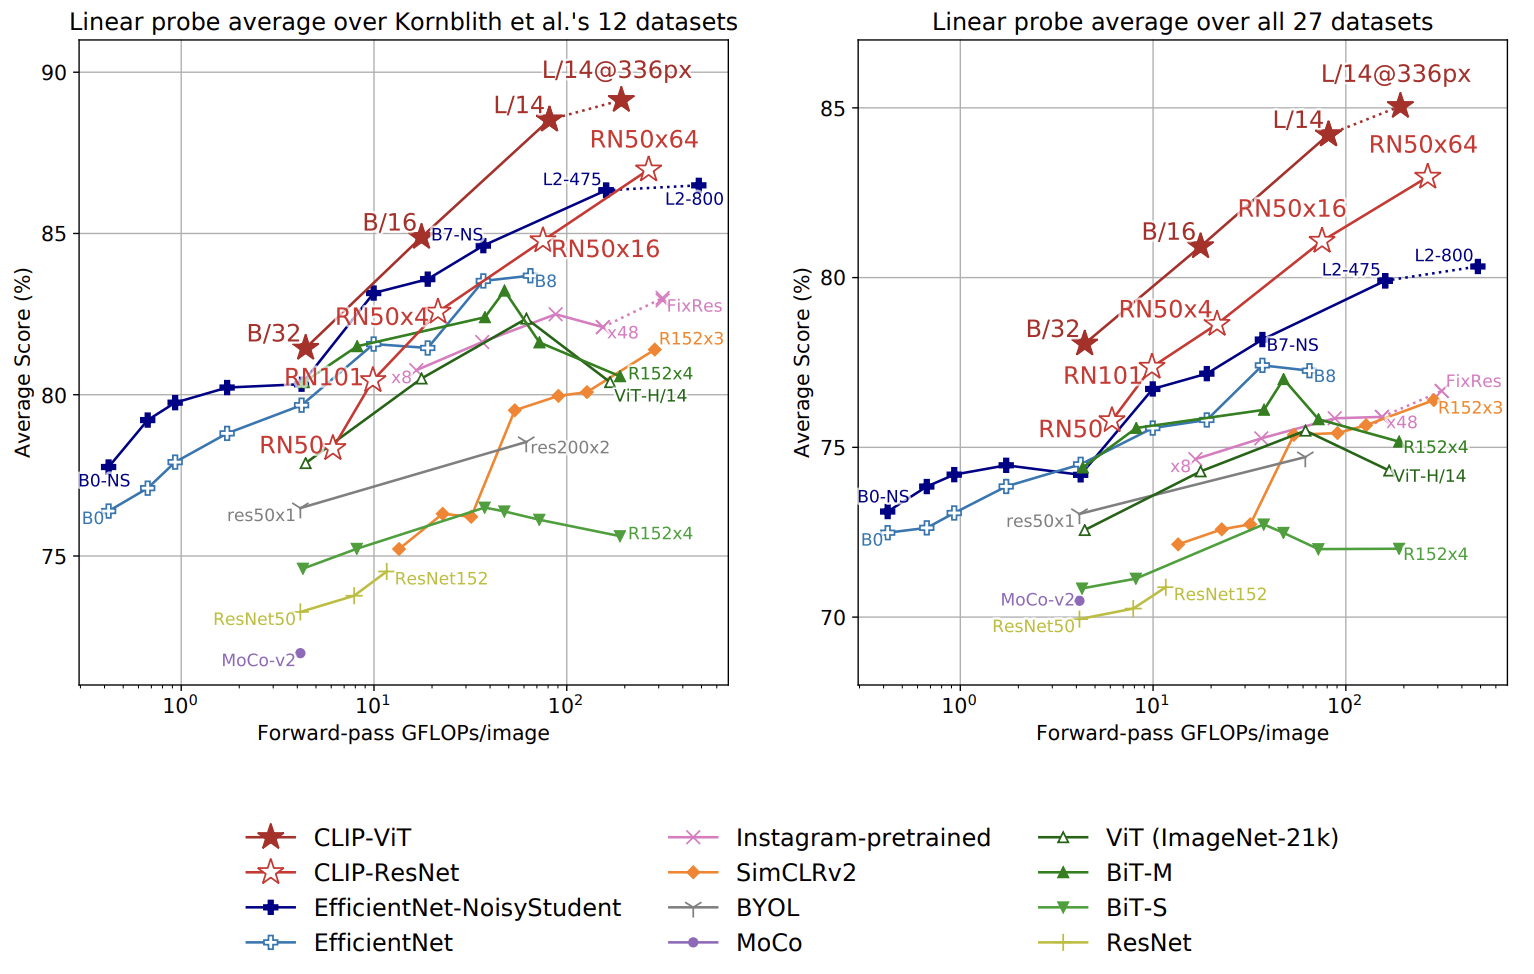
\includegraphics[width=0.75 \linewidth]{figures/representation_learning_capability.png}
        \label{representation_learning_capability}
    \end{figure}    
\end{frame}

%------------------------------------------------

\begin{frame}{Analysis - Representation Learning}
    \begin{itemize}
        \item the largest CLIP model slightly outperforms the best existing model on both overall score and compute efficiency
        \item CLIP transformers 3x more compute efficient than CLIP ResNets
        \bigskip
        \textbf{Broader evaluation suite} tasks include geo-localization, optical character recognition, facial emotion recognition, and character recognition
        \begin{itemize}
            \item All CLIP models, regardless of scale, outperform all evaluated systems in terms of compute efficiency
        \end{itemize}
    \end{itemize}
\end{frame}

%------------------------------------------------

\begin{frame}{Analysis -  Distribution shift}
    \begin{figure}
        \centering
        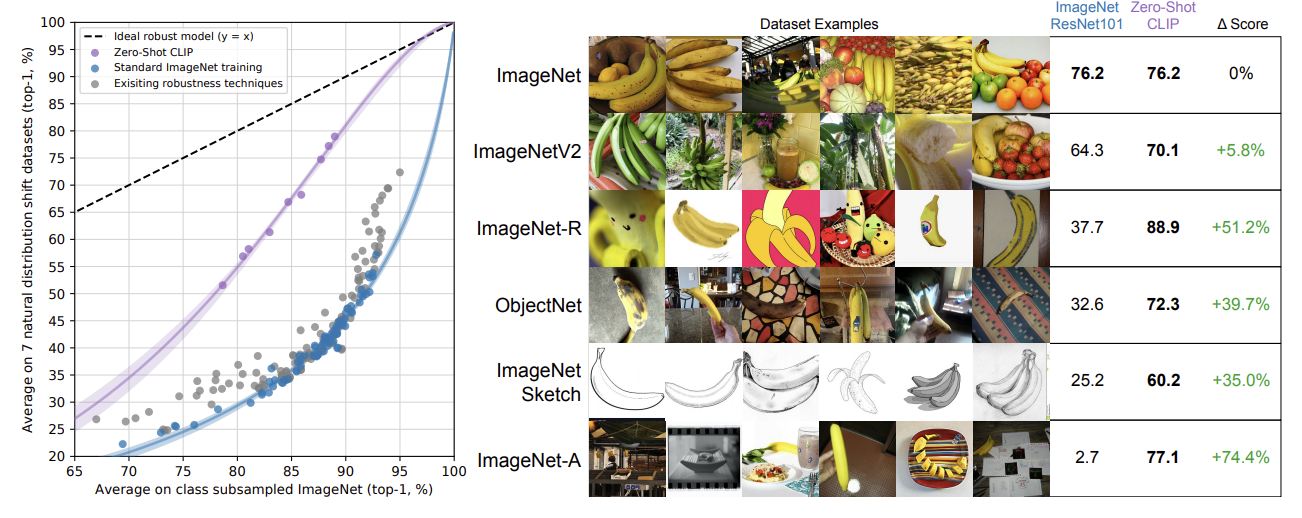
\includegraphics[width=0.75 \linewidth]{figures/distribution_shift.png}
        \label{distribution_shift}
    \end{figure}   
    Zero-shot CLIP is much more robust to distribution shift than the ResNet101.\\
\end{frame}

%------------------------------------------------

\begin{frame}
    \Huge{\centerline{\textbf{The End}}}
\end{frame}

%----------------------------------------------------------------------------------------

\end{document}